\documentclass[11pt]{article}

\usepackage[T1]{fontenc}
\usepackage[utf8]{inputenc}
\usepackage{lmodern}
\usepackage{microtype}
\usepackage[margin=1in]{geometry}
\usepackage{amsmath}
\usepackage{amssymb}
\usepackage{graphicx}
\usepackage{booktabs}
\usepackage{tabularx}
\usepackage{longtable}
\usepackage{array}
\usepackage{url}
\usepackage{cite}
\usepackage[colorlinks=true,linkcolor=blue,citecolor=blue,urlcolor=blue]{hyperref}

\graphicspath{{figures/}}

\title{Evaluating Open-Set Reliability in Leukocyte Morphology Classification under Domain Shift}
\author{G. Álvarez Sánchez}
\date{}

\begin{document}
\maketitle

\begin{abstract}
Automated leukocyte morphology classifiers are commonly evaluated under a closed-set assumption, although deployed or reused models may encounter morphologies outside the training taxonomy. We evaluated whether high closed-set performance implies reliable rejection of unseen morphologies under internal and external domain shift. The known taxonomy comprised basophils, eosinophils, lymphocytes, monocytes, and segmented neutrophils. In MLL23, 12,793 known images were used for training, 2,741 for validation, 2,742 for known testing, and 23,345 held-out images from 13 morphologies for unknown testing. ImageNet-pretrained ResNet18 models trained with cross entropy or ArcFace were assessed across five seeds and two split protocols using post-hoc open-set scores. Internal closed-set macro-F1 was high for both losses, approximately 0.97. Internal open-set recognition was lower: CE+ViM achieved AUROC 0.877 $\pm$ 0.004 on V1 and 0.874 $\pm$ 0.008 on the near-duplicate-aware V2 sensitivity split, with FPR@95TPR 0.484 $\pm$ 0.027 and 0.528 $\pm$ 0.050. On AML-Cytomorphology\_LMU, an independent 18,365-image test-only dataset, performance degraded substantially; external AUROC ranged from 0.563 to 0.696 on V1 systems and from 0.573 to 0.696 on V2 systems, with high FPR@95TPR. Failure was morphology-dependent, with neutrophil-band, monoblast, myeloblast, and atypical lymphocyte among the hardest external unknowns. ArcFace improved some known-class geometry summaries but did not reproduce as a robust superior open-set representation. Persistent-homology analyses were negative or explanatory rather than predictive. Strong closed-set leukocyte classification therefore did not ensure reliable unseen-morphology rejection, especially under morphological similarity and external domain shift.
\end{abstract}


\noindent\textbf{Keywords:} open-set recognition; leukocyte morphology; domain shift; out-of-distribution detection; hematological image analysis; external validation

\section{Introduction}

Microscopic leukocyte morphology remains a central source of information in hematology. Expert review of peripheral blood and bone marrow smears supports differential counts, quality control of automated analyzers, and recognition of morphologies that may warrant further laboratory interpretation. In parallel, convolutional neural networks and related image-analysis methods have achieved high accuracy on curated blood-cell image datasets, including peripheral blood and bone marrow morphology collections \cite{walter2023_ai_hematology,khan2021_wbc_review,deshpande2021_blood_cells_review,acevedo2019_peripheral_blood_cnn,matek2019_blast,matek2021_bone_marrow}. These advances make automated morphology recognition a strong research problem for biomedical image analysis. They also create a methodological risk: closed-set performance can look convincing even when the evaluation never asks what happens to cells outside the training taxonomy.

The conventional closed-set setting assumes that every test image belongs to one of the classes seen during training. That assumption is convenient for supervised learning, but it is fragile for morphology recognition. A model trained on mature leukocyte categories can encounter immature, atypical, rare, damaged, or otherwise out-of-taxonomy cells at test time. If evaluation forces every such image into one of the known classes, the model may appear confident while performing the wrong kind of task. Open-set recognition addresses this gap by requiring a system both to classify known samples and to reject samples from unseen classes \cite{scheirer2013_open_set,geng2021_osr_survey,bendale2016_openmax,yang2024_generalized_ood}. In the present study, the open-set question is deliberately narrow: can a classifier trained on a fixed leukocyte morphology taxonomy identify that a test image should not be assigned to that taxonomy?

This distinction is especially important because ``unknown'' has a technical meaning here. The known classes are basophil, eosinophil, lymphocyte, monocyte, and segmented neutrophil. An unknown sample is a morphology outside that training taxonomy. It is not a cancer label, leukemia label, malignant label, abnormal diagnosis, patient-level endpoint, or clinically positive finding. The work therefore should not be read as a diagnostic system or leukemia detector. It is an empirical study of recognition reliability when the model's label inventory is incomplete.

The hardest unknown samples are often not visually alien. A band neutrophil is close to segmented neutrophils; a monoblast can be pulled toward monocytes; blast or atypical lymphoid morphologies can resemble the neighborhood of typical lymphocytes. Such examples are not merely generic outliers. They are near-taxonomy morphologies whose errors may be structured by cell lineage, maturation, image acquisition, and representation geometry. This makes leukocyte open-set recognition a demanding biomedical image-analysis problem: the model must reject samples that are related to, but not members of, the known classes.

External domain shift compounds the problem. Hematology image datasets can differ in staining, scanner, objective, cropping, annotation policy, patient mix, image size, and class composition. Prior work in medical image analysis and blood-cell classification has shown that models trained and tested under similar imaging conditions can lose performance when evaluated across sources \cite{guan2022_domain_adaptation_medical,litjens2017_medical_ai_survey,salehi2022_cross_domain,sadafi2024_continual_wbc,tsutsui2023_wbc_domain_shift}. For open-set recognition, external validation is even more demanding because both known-class classification and unknown rejection can change simultaneously. A score that is stable internally may no longer rank methods correctly in a new acquisition domain.

Despite extensive work on leukocyte classification and growing work on open-set and out-of-distribution detection, evidence remains limited for protocols that explicitly hold out named hematological morphologies as unknown classes, evaluate multiple seeds, preserve unknowns as test-only data, and test whether internal rankings transfer to an external hematology dataset. This gap motivates the present manuscript. We evaluate a frozen open-set protocol using MLL23 as the internal domain and AML-Cytomorphology\_LMU as an independent test-only domain \cite{mll23_nature_2025,mll23_zenodo_2024,aml_lmu_tcia_2019}. The scientific thesis is that high closed-set leukocyte morphology classification performance does not imply reliable open-set recognition of unseen morphologies, particularly under morphological similarity and external domain shift.

The contributions are:
\begin{itemize}
\item A reproducible open-set evaluation protocol for leukocyte morphology recognition, with a frozen five-class known taxonomy and held-out MLL23 morphologies used only for open-set testing.
\item A five-seed and two-split sensitivity analysis showing that internal closed-set macro-F1 near 0.97 coexists with imperfect unknown rejection and high FPR@95TPR.
\item An external test-only AML-Cytomorphology\_LMU validation showing substantial domain-shift degradation and instability of internal method rankings.
\item A morphology-level failure analysis showing that difficult unknown rejection is structured by known-class attractors such as band-to-segmented neutrophil, monoblast-to-monocyte, and lymphoid-to-lymphocyte.
\item Controlled negative or secondary evidence showing that improved known-class geometry and persistent-homology descriptors do not automatically translate into robust open-set recognition.
\end{itemize}

\begin{figure}[htbp]
\centering
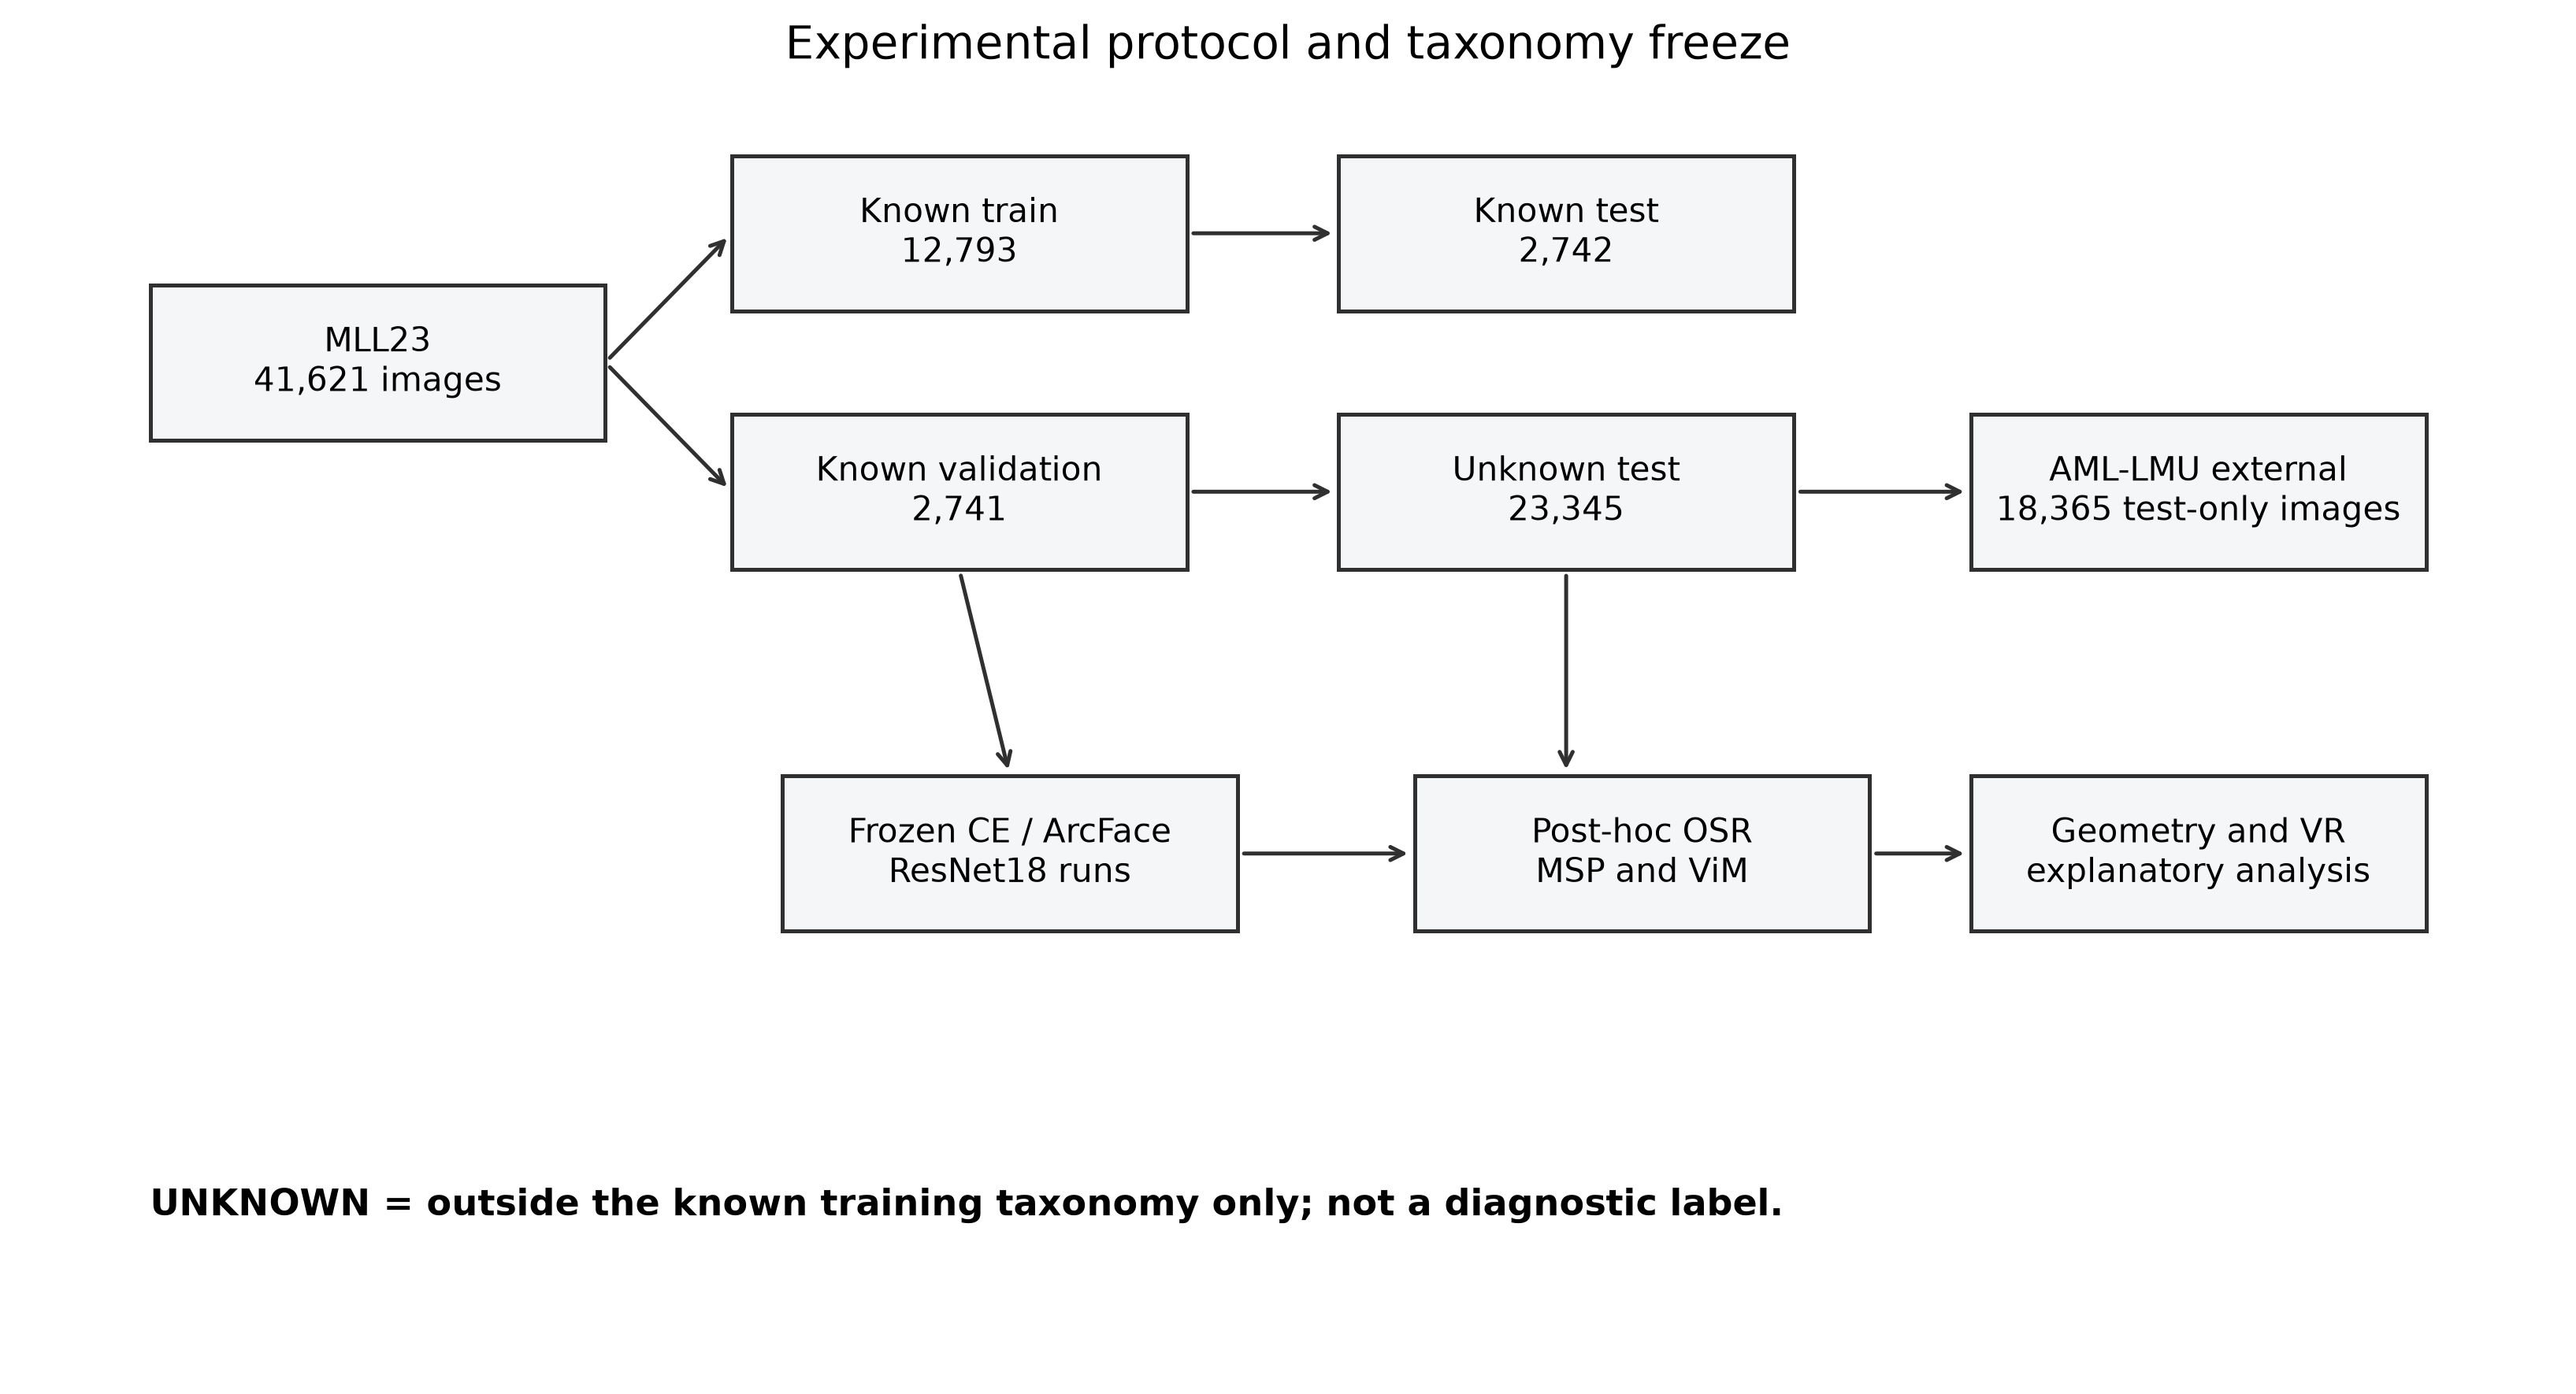
\includegraphics[width=\textwidth]{figure1_protocol.png}
\caption{Frozen open-set evaluation protocol. MLL23 is used for internal multiseed evaluation, with five mature leukocyte classes treated as known and 13 morphologies held out as unknown. AML-Cytomorphology\_LMU is used only as an external test domain, without training, tuning, calibration, or representation fitting.}
\label{fig:protocol}
\end{figure}

\section{Related Work}

\subsection{Automated Leukocyte Morphology Classification}

Automated blood-cell image analysis has a long history, but recent progress has been driven by annotated single-cell datasets and convolutional neural networks. Reviews of white blood cell classification report a broad literature on segmentation, feature extraction, transfer learning, and deep classifiers for microscopic blood-smear imagery \cite{khan2021_wbc_review,deshpande2021_blood_cells_review}. Much of this work evaluates a fixed set of classes and reports accuracy, precision, recall, or F1 score under same-dataset splits. Such studies are useful for establishing classification feasibility, but they generally do not test whether a model can refuse a sample outside its label inventory.

Several influential hematology image-analysis studies demonstrate the strength of deep learning under closed-set or task-specific settings. Acevedo et al. introduced a peripheral blood cell dataset and reported convolutional recognition of multiple cell categories \cite{acevedo2019_peripheral_blood_cnn}. Matek et al. showed high-performance blast-cell recognition in acute myeloid leukemia images and later extended deep learning to large bone marrow morphology classification \cite{matek2019_blast,matek2021_bone_marrow}. Walter et al. review the broader promise and limitations of artificial intelligence in hematological diagnostics \cite{walter2023_ai_hematology}. These studies establish the relevance of automated morphology analysis but do not remove the need for open-set evaluation. Strong classification of known cell types is a different claim from reliable rejection of unseen morphologies.

This distinction matters because morphology labels are not interchangeable with patient-level clinical endpoints. A smear image can be assigned a cell-type or maturation label without determining the patient's diagnosis, and a model can be useful for one of these tasks while being inappropriate for the other. The present manuscript therefore keeps the task at the single-cell morphology level. Its central question is not whether a patient has leukemia or whether a sample is clinically abnormal, but whether a classifier trained on mature leukocytes can recognize when an image belongs outside that fixed label inventory. That framing follows the data available in the frozen artifacts and avoids translating morphology rejection into a diagnostic claim that the experiments do not test.

The MLL23 dataset is particularly relevant because it contains more than 40,000 expert-annotated single-cell images in 18 morphologically defined classes, with 288 by 288 pixel TIFF images after curation \cite{mll23_nature_2025,mll23_zenodo_2024}. Its class diversity makes it possible to define an explicit open-set protocol by training on mature leukocytes and holding out other named morphologies. The AML-Cytomorphology\_LMU collection is also central because it provides an independent TCIA source with 18,365 expert-labeled single-cell images from peripheral blood smears \cite{aml_lmu_tcia_2019}. The combination of MLL23 and AML-LMU allows the paper to ask not only whether unknown morphologies can be rejected internally, but whether the same conclusions survive external acquisition differences.

\subsection{Open-Set Recognition and Out-of-Distribution Detection}

Open-set recognition was formalized to address settings where not all test classes are known during training \cite{scheirer2013_open_set}. In deep learning, OpenMax showed that closed-set neural networks can assign high confidence to inputs outside the training taxonomy and introduced a recalibrated output layer for unknown rejection \cite{bendale2016_openmax}. Surveys of open-set recognition emphasize that the task requires balancing known-class recognition with unknown-class rejection, and that evaluation protocols must avoid using unknown-test data during method selection \cite{geng2021_osr_survey}.

Out-of-distribution detection is closely related but not identical. Generalized OOD surveys unify anomaly detection, novelty detection, open-set recognition, OOD detection, and outlier detection while highlighting differences in training assumptions and semantic shift \cite{yang2024_generalized_ood}. In medical image analysis, OOD detection is especially important because models may encounter unseen pathologies, acquisition changes, artifacts, or population differences \cite{hong2024_medical_ood_survey}. The present study lies at the overlap of open-set recognition and medical OOD detection: the unknown samples are semantic morphology classes held out from training, while external AML-LMU evaluation also introduces acquisition and taxonomy-domain differences.

Several post-hoc OOD scores are relevant baselines. Maximum softmax probability remains a strong and simple method because closed-set confidence is often informative even when imperfect \cite{hendrycks2017_msp}. Energy scores use the log-sum-exp of logits to reduce reliance on the top softmax probability alone \cite{liu2020_energy}. ReAct clips internal activations to reduce overconfident behavior on OOD inputs \cite{sun2021_react}. ViM combines a feature-space residual term with logit evidence through virtual-logit matching \cite{wang2022_vim}. These methods differ in what they fit after training, so leakage control matters. Fitting PCA subspaces, centroids, covariance estimates, or clipping thresholds with unknown-test data would invalidate an open-set evaluation.

The leakage issue is especially subtle in biomedical studies because the same external dataset can easily become both a validation resource and a reported test resource. For example, choosing a threshold, selecting a score family, deciding whether to normalize stains, or fitting a feature residual subspace after looking at external labels can improve apparent performance while changing the scientific question. Such choices may be appropriate in a deployment-engineering study, but they no longer measure zero-shot transfer of the frozen internal protocol. The present manuscript therefore treats post-hoc scoring as part of the internal pipeline and keeps AML-LMU completely outside all fitting and selection steps.

\subsection{Representation Learning and Unknown Rejection}

Representation learning can improve known-class embedding geometry. Supervised contrastive learning encourages samples from the same class to cluster while separating samples from different classes \cite{khosla2020_supcon}. ArcFace imposes an angular margin between normalized features and normalized class weights and has been highly influential in face recognition \cite{deng2019_arcface}. In principle, tighter known-class clusters and larger inter-class margins could improve open-set rejection because unknown samples might lie farther from all known classes.

That hypothesis is plausible but not guaranteed. Unknown morphologies can be visually close to known classes, and a representation that improves known-class compactness may also make near-taxonomy unknowns more confidently attracted to a known prototype. For this reason, representation-learning results must be judged by multiseed and split sensitivity, not by a single favorable run. The present manuscript treats ArcFace as a major ablation and asks whether its internal gains reproduce across seeds, splits, and external validation. It does not present ArcFace as a newly proposed hematology method.

\subsection{Domain Shift and External Validation in Medical Imaging}

Domain shift is a persistent obstacle in medical image analysis. Differences in scanners, staining, acquisition protocols, preprocessing, patient populations, and annotation conventions can all degrade model performance outside the source dataset \cite{litjens2017_medical_ai_survey,guan2022_domain_adaptation_medical}. In blood-cell morphology, cross-domain classification studies have reported that performance can drop when testing across datasets or imaging sources \cite{salehi2022_cross_domain,sadafi2024_continual_wbc,tsutsui2023_wbc_domain_shift}. Such evidence is important because many closed-set benchmarks overestimate generalization when train and test images come from the same source.

External validation is even more stringent in open-set recognition. A model may face both covariate shift among known classes and semantic shift in the unknown set. A post-hoc score that ranks known and unknown samples well internally may fail when known samples from the new domain acquire lower confidence or when unknown samples resemble known classes in a different way. This motivates the test-only AML-LMU design: no external data are used to adapt the model, tune thresholds, choose scorers, fit PCA residuals, or adjust preprocessing. The external result therefore measures the generalization of the frozen internal protocol rather than the success of external adaptation.

This choice also shapes how negative results should be interpreted. A poor external AUROC is not evidence that adaptation would be impossible, and a high FPR@95TPR is not a final clinical operating point. Instead, these results quantify how much reliability remains when a closed-set morphology classifier and its post-hoc open-set scores are transferred without external assistance. In that sense, the external experiment is closer to an audit of robustness than to an optimization benchmark. It asks whether internal model ranking is trustworthy when the data source changes, which is a practical concern for biomedical image-analysis papers that report only same-source splits.

\subsection{Topological Analysis of Learned Representations}

Persistent homology summarizes connected components, loops, and higher-dimensional features across filtrations \cite{edelsbrunner2002_persistence,carlsson2009_topology}. Computational libraries such as GUDHI support cubical and simplicial constructions for images and point clouds \cite{maria2014_gudhi}. In biomedical image analysis, topology can be used either as a feature representation or as a descriptive lens on learned embeddings. These two roles should not be conflated.

This manuscript keeps topology secondary. Cubical persistent homology is evaluated as a predictive ablation over image-derived filtrations and fusion designs. Vietoris-Rips persistent homology is used only after the predictive experiments are frozen, to describe embedding-cloud geometry across known and hard unknown morphologies. The resulting evidence is useful because it prevents overclaiming: the topology results support negative and explanatory conclusions, not a new topology-based open-set method.

\section{Materials and Methods}

\subsection{Datasets}

\subsubsection{MLL23 Internal Domain}

MLL23 is the internal dataset for model training, known-validation checkpoint selection, known testing, and internal unknown testing \cite{mll23_nature_2025,mll23_zenodo_2024}. The audited manifest used in this study contains 41,621 TIFF images, each 288 by 288 pixels, assigned to 18 canonical morphology classes. The known training taxonomy is restricted to five mature leukocyte classes: basophil, eosinophil, lymphocyte, monocyte, and segmented neutrophil. The remaining 13 MLL23 morphologies are held out as unknown classes and are not used for training, validation, calibration, representation fitting, or model selection.

The frozen split counts are 12,793 known-training images, 2,741 known-validation images, 2,742 known-test images, and 23,345 unknown-test images. Known-validation samples are used only for checkpoint selection based on known-class macro-F1 and for threshold-related reporting where a threshold is needed. Unknown-test samples are reserved for final metric computation and morphology-level failure analysis. Exact sample identifiers and checksums are not allowed to cross train/test boundaries.

The known-validation role is intentionally narrow. It supports model selection among checkpoints produced from the same training run, but it does not supply unknown examples for tuning an open-set decision boundary. This design avoids a common ambiguity in open-set studies: if held-out unknown morphologies are used to choose a threshold or score family, they are no longer fully unseen for evaluation. The frozen protocol therefore separates known-class checkpointing from unknown-class testing.

\subsubsection{AML-Cytomorphology\_LMU External Domain}

AML-Cytomorphology\_LMU is the independent external validation dataset \cite{aml_lmu_tcia_2019}. The audited manifest contains 18,365 TIFF images that load as 400 by 400 RGB arrays. The collection documents expert-labeled single-cell peripheral blood smear images from 100 patients diagnosed with acute myeloid leukemia and 100 non-malignant controls. Patient identifiers were not available in the audited API fields or annotation file used by this project; therefore, no patient-level split is claimed.

The external taxonomy mapping was frozen before evaluation. BAS, EOS, LYT, MON, and NGS map to basophil, eosinophil, lymphocyte, monocyte, and segmented neutrophil, respectively. EBO, KSC, LYA, MMZ, MOB, MYB, MYO, NGB, PMB, and PMO are treated as external unknown morphologies. UNC and missing re-annotation labels are excluded by policy and have zero samples in the audited gold-standard column. Band neutrophils are not collapsed into segmented neutrophils, atypical lymphocytes are not collapsed into typical lymphocytes, and blast or immature labels are not encoded as mature known classes.

AML-LMU is test-only. It is never used for external fine-tuning, threshold calibration, method selection, PCA fitting, ViM fitting, kNN reference construction, external preprocessing selection, or taxonomy revision. This restriction is a major design feature: the external experiment evaluates frozen internal systems under domain shift.

Because AML-LMU contains both mapped known classes and mapped unknown morphologies, it can test two behaviors at once. The closed-set portion measures whether known mature leukocytes transfer across domains. The open-set portion measures whether out-of-taxonomy morphologies remain separable from the known classes under the same transfer. The two behaviors are reported separately because a model can preserve one while losing the other.

\begin{table}[htbp]
\centering
\small
\begin{tabularx}{\textwidth}{l l r r r l X}
\toprule
Dataset & Role & Images & Known & Unknown & Format & Use in protocol \\
\midrule
MLL23 & Internal & 41,621 & 5 & 13 & TIFF, 288$\times$288 & Known classes are used for training, validation, and known testing; held-out morphologies are test-only unknowns. \\
AML-LMU & External & 18,365 & 5 mapped & 10 mapped & TIFF, 400$\times$400 RGB & Test-only external validation; no adaptation, calibration, threshold tuning, PCA fitting, ViM fitting, or method selection. \\
\bottomrule
\end{tabularx}
\caption{Datasets and open-set protocol roles. Unknown denotes only outside the known training taxonomy; it is not a diagnostic label.}
\label{tab:datasets}
\end{table}


\subsection{Open-Set Taxonomy and Split Protocols}

Let $\mathcal{Y}_K$ denote the known training taxonomy:
\[
\mathcal{Y}_K = \{\text{basophil}, \text{eosinophil}, \text{lymphocyte}, \text{monocyte}, \text{neutrophil\_segmented}\}.
\]
For a test image $x$, the closed-set classifier predicts one class in $\mathcal{Y}_K$. Open-set evaluation additionally asks whether $x$ belongs outside $\mathcal{Y}_K$. Unknown is therefore a protocol status, not a diagnosis.

Two internal split protocols are evaluated. V1 is the deterministic original split. V2 is a conservative near-duplicate-aware sensitivity split based on exact checksum and perceptual-hash candidate audits. The V2 audit preserves the same split totals while resolving high-confidence grouped cross-split candidates. Because reliable patient or acquisition-group identifiers were unavailable in the working MLL23 manifests, V2 is not described as patient-independent validation. It is a sensitivity analysis for exact and near-duplicate leakage, not a substitute for patient-level validation.

\subsection{Backbone, Preprocessing, and Training}

The principal model family is an ImageNet-pretrained ResNet18 \cite{he2016_resnet}. Images are resized to 224 by 224 pixels and normalized according to the frozen training pipeline. The network outputs logits for the five known classes and a 512-dimensional pre-logit embedding. Training uses AdamW with learning rate $3\times10^{-4}$, weight decay $10^{-4}$, batch size 64, automatic mixed precision, and checkpoint selection by known-validation macro-F1. The main experiments are repeated over five seeds: 13, 37, 73, 101, and 137.

The baseline representation uses cross-entropy training. The ArcFace ablation uses normalized features and normalized class weights. If $z$ is the embedding and $w_c$ is the class weight for class $c$, then
\[
\hat{z}=\frac{z}{\lVert z\rVert}, \qquad
\hat{w}_c=\frac{w_c}{\lVert w_c\rVert}, \qquad
\cos\theta_c=\hat{w}_c^\top \hat{z}.
\]
For the target class $y$, the training logit is $s\cos(\theta_y+m)$ with fixed scale $s=30$ and margin $m=0.30$. No target margin is applied at inference because the target label is unknown. ArcFace configuration is frozen before multiseed confirmation.

\subsection{Post-Hoc Open-Set Scores}

For input $x$, let $f_c(x)$ be the logit for class $c\in\mathcal{Y}_K$. The closed-set prediction is
\[
\hat{y}(x)=\arg\max_{c\in\mathcal{Y}_K} f_c(x).
\]
Each post-hoc open-set method defines an unknownness score $S(x)$ oriented so that larger values indicate stronger evidence that $x$ lies outside $\mathcal{Y}_K$.

Maximum softmax probability (MSP) uses the negative maximum softmax confidence as the unknownness score \cite{hendrycks2017_msp}. Energy uses an oriented log-sum-exp score \cite{liu2020_energy}. Cosine kNN uses the mean cosine distance to the $k=5$ nearest known-training embeddings. Nearest-class-mean and Mahalanobis scores compare embeddings with class prototypes or covariance-normalized residuals fitted on known-training embeddings. ReAct clips pre-classifier activations using a known-training percentile and recomputes an energy-like score \cite{sun2021_react}. ViM fits a known-training PCA residual subspace and combines residual magnitude with logit evidence through virtual-logit matching \cite{wang2022_vim}. All fitted quantities are derived from known-training data only.

These scores represent common families of post-hoc open-set evidence. Confidence-based scores ask whether the classifier is uncertain among known classes. Distance-based scores ask whether an embedding is far from the known training distribution. Residual-subspace scores ask whether an embedding contains components poorly explained by known-class variation. These families can disagree, particularly under domain shift. The manuscript therefore reports MSP and ViM as principal comparators rather than selecting a winner after inspecting AML-LMU labels.

\subsection{Evaluation Metrics and Statistical Reporting}

Closed-set accuracy is the proportion of known-test samples whose predicted class equals the label. Balanced accuracy is the average of per-class recalls across known classes. Macro-F1 is the unweighted mean of per-class F1 scores. These metrics are reported for known-class classification because external class imbalance can make aggregate accuracy overly optimistic.

Open-set metrics compare known-test samples with unknown-test samples. Unless otherwise stated, unknown samples are treated as the positive class. AUROC is the area under the receiver-operating-characteristic curve obtained by thresholding $S(x)$. AUPR is reported with both known and unknown orientation in artifacts, but the main manuscript emphasizes unknown-positive open-set behavior. FPR@95TPR is the false-positive rate among known samples when the true-positive rate for unknown samples is fixed at 95\%. OSCR summarizes the tradeoff between correct known classification and unknown rejection; it is retained in tables but not used to introduce new result selection.

FPR@95TPR is intentionally stringent. It answers a different question from AUROC: if the system is forced to catch most unknown samples, how many known samples would be incorrectly rejected? In the present task, high FPR@95TPR should not be interpreted as a chosen clinical threshold. It is a standardized stress metric that makes the cost of high unknown sensitivity visible. Macro-F1 and FPR@95TPR are therefore complementary: the former describes known-class recognition, whereas the latter describes the burden of maintaining high unknown detection.

All multiseed main results are reported as mean $\pm$ standard deviation over five seeds. Paired CE-versus-ArcFace statements use the frozen matched-seed delta summaries where available. The manuscript avoids post-hoc p-values and uses conservative language such as higher, lower, consistent, not consistently reproduced, interval includes zero, or favorable in $x/5$ seeds.

No inferential test is added after the fact. This is deliberate because the study was not planned around a formal null-hypothesis testing hierarchy, and the frozen evidence is better summarized as multiseed stability, direction consistency, and external transfer. When a pattern changes between V1 and V2, the manuscript treats that change as evidence against robust superiority rather than as an opportunity to select the more favorable split.

\subsection{Morphology-Dependent Failure Analysis}

Morphology-level analysis is performed after aggregate metrics are frozen. For each unknown morphology, AUROC and FPR@95TPR are computed against the known-test distribution. Known-class attractors are estimated by the dominant closed-set prediction assigned to unknown samples. This analysis is descriptive: it identifies recognition-space failure patterns, not biological causality or diagnostic status.

\subsection{Persistent-Homology Analyses}

Cubical persistent homology is evaluated as a predictive ablation over image-derived filtrations, including raw grayscale fields, morphology-candidate distance maps, and CNN feature-map filtrations. Vectorized persistence features and fusion designs are fitted with training-only statistics. These experiments test whether persistent-homology summaries add predictive open-set signal beyond deep embeddings.

Vietoris-Rips persistent homology is used only as an explanatory embedding analysis. For a point cloud $X=\{z_1,\ldots,z_n\}$ of L2-normalized embeddings with cosine distance $d$, the Vietoris-Rips complex at scale $\epsilon$ is
\[
VR_\epsilon(X)=\{\sigma\subseteq X: d(z_i,z_j)\leq \epsilon\ \forall z_i,z_j\in\sigma\}.
\]
The frozen analysis uses GUDHI 3.13.0, 192 samples per cloud, a fixed sample seed, and $H_0$ and $H_1$ summaries. These summaries are not used for training, thresholding, prediction, or method selection.

\subsection{Reproducibility and Leakage Controls}

The manuscript is organized around a result freeze rather than a new result-selection phase. Headline values are recorded in \texttt{results\_freeze.yaml}, and numerical claims in the abstract, results, discussion, and conclusion are indexed in \texttt{claim\_traceability.csv}. The traceability file links each quantitative statement to a frozen artifact, row filter, value, and verification status.

Several controls preserve the open-set interpretation. Unknown morphologies are declared before metrics are produced. Unknown samples are absent from training, known-validation checkpointing, calibration, representation fitting, and method selection. External AML-LMU data are absent from all fitting steps. The V2 split is labeled only as an exact and near-duplicate sensitivity analysis because patient-level identifiers are unavailable. These controls do not make the protocol clinically complete, but they prevent the most direct forms of information leakage for the research question studied here.

\section{Results}

\subsection{Closed-Set Performance on Known Morphologies}

Internal closed-set classification was consistently strong across the five known mature leukocyte classes. With cross-entropy training, closed-set macro-F1 was 0.970 $\pm$ 0.004 on V1 and 0.970 $\pm$ 0.004 on V2. With ArcFace, closed-set macro-F1 was 0.970 $\pm$ 0.004 on V1 and 0.969 $\pm$ 0.005 on V2. These values show that the ResNet18 family learned the known morphology taxonomy well under both split protocols. They do not, however, establish reliable open-set behavior because the closed-set calculation excludes held-out unknown morphologies.

\subsection{Internal Open-Set Recognition}

Internal open-set performance was substantially lower than closed-set classification. CE+MSP achieved AUROC 0.868 $\pm$ 0.014 on V1 and 0.872 $\pm$ 0.019 on V2. CE+ViM achieved AUROC 0.877 $\pm$ 0.004 on V1 and 0.874 $\pm$ 0.008 on V2. The smaller standard deviation of CE+ViM supports its role as the most stable internal comparator, but FPR@95TPR remained high: 0.484 $\pm$ 0.027 on V1 and 0.528 $\pm$ 0.050 on V2. Thus, even the strongest internal comparator would falsely flag a substantial proportion of known samples when unknown sensitivity is fixed at 95\%.

\begin{table}[htbp]
\centering
\small
\resizebox{\textwidth}{!}{%
\begin{tabular}{l c c c c c c}
\toprule
System & V1 AUROC & V1 FPR@95TPR & V1 closed F1 & V2 AUROC & V2 FPR@95TPR & V2 closed F1 \\
\midrule
CE+MSP & 0.868 $\pm$ 0.014 & 0.515 $\pm$ 0.061 & 0.970 $\pm$ 0.004 & 0.872 $\pm$ 0.019 & 0.530 $\pm$ 0.103 & 0.970 $\pm$ 0.004 \\
CE+ViM & 0.877 $\pm$ 0.004 & 0.484 $\pm$ 0.027 & 0.970 $\pm$ 0.004 & 0.874 $\pm$ 0.008 & 0.528 $\pm$ 0.050 & 0.970 $\pm$ 0.004 \\
ArcFace+MSP & 0.881 $\pm$ 0.012 & 0.445 $\pm$ 0.046 & 0.970 $\pm$ 0.004 & 0.852 $\pm$ 0.030 & 0.537 $\pm$ 0.064 & 0.969 $\pm$ 0.005 \\
ArcFace+ViM & 0.869 $\pm$ 0.014 & 0.543 $\pm$ 0.062 & 0.970 $\pm$ 0.004 & 0.850 $\pm$ 0.025 & 0.611 $\pm$ 0.086 & 0.969 $\pm$ 0.005 \\
\bottomrule
\end{tabular}
}
\caption{Internal MLL23 multiseed results. Values are mean $\pm$ standard deviation over five training seeds. Unknown samples are positive for AUROC and FPR@95TPR.}
\label{tab:internal}
\end{table}


\begin{figure}[htbp]
\centering
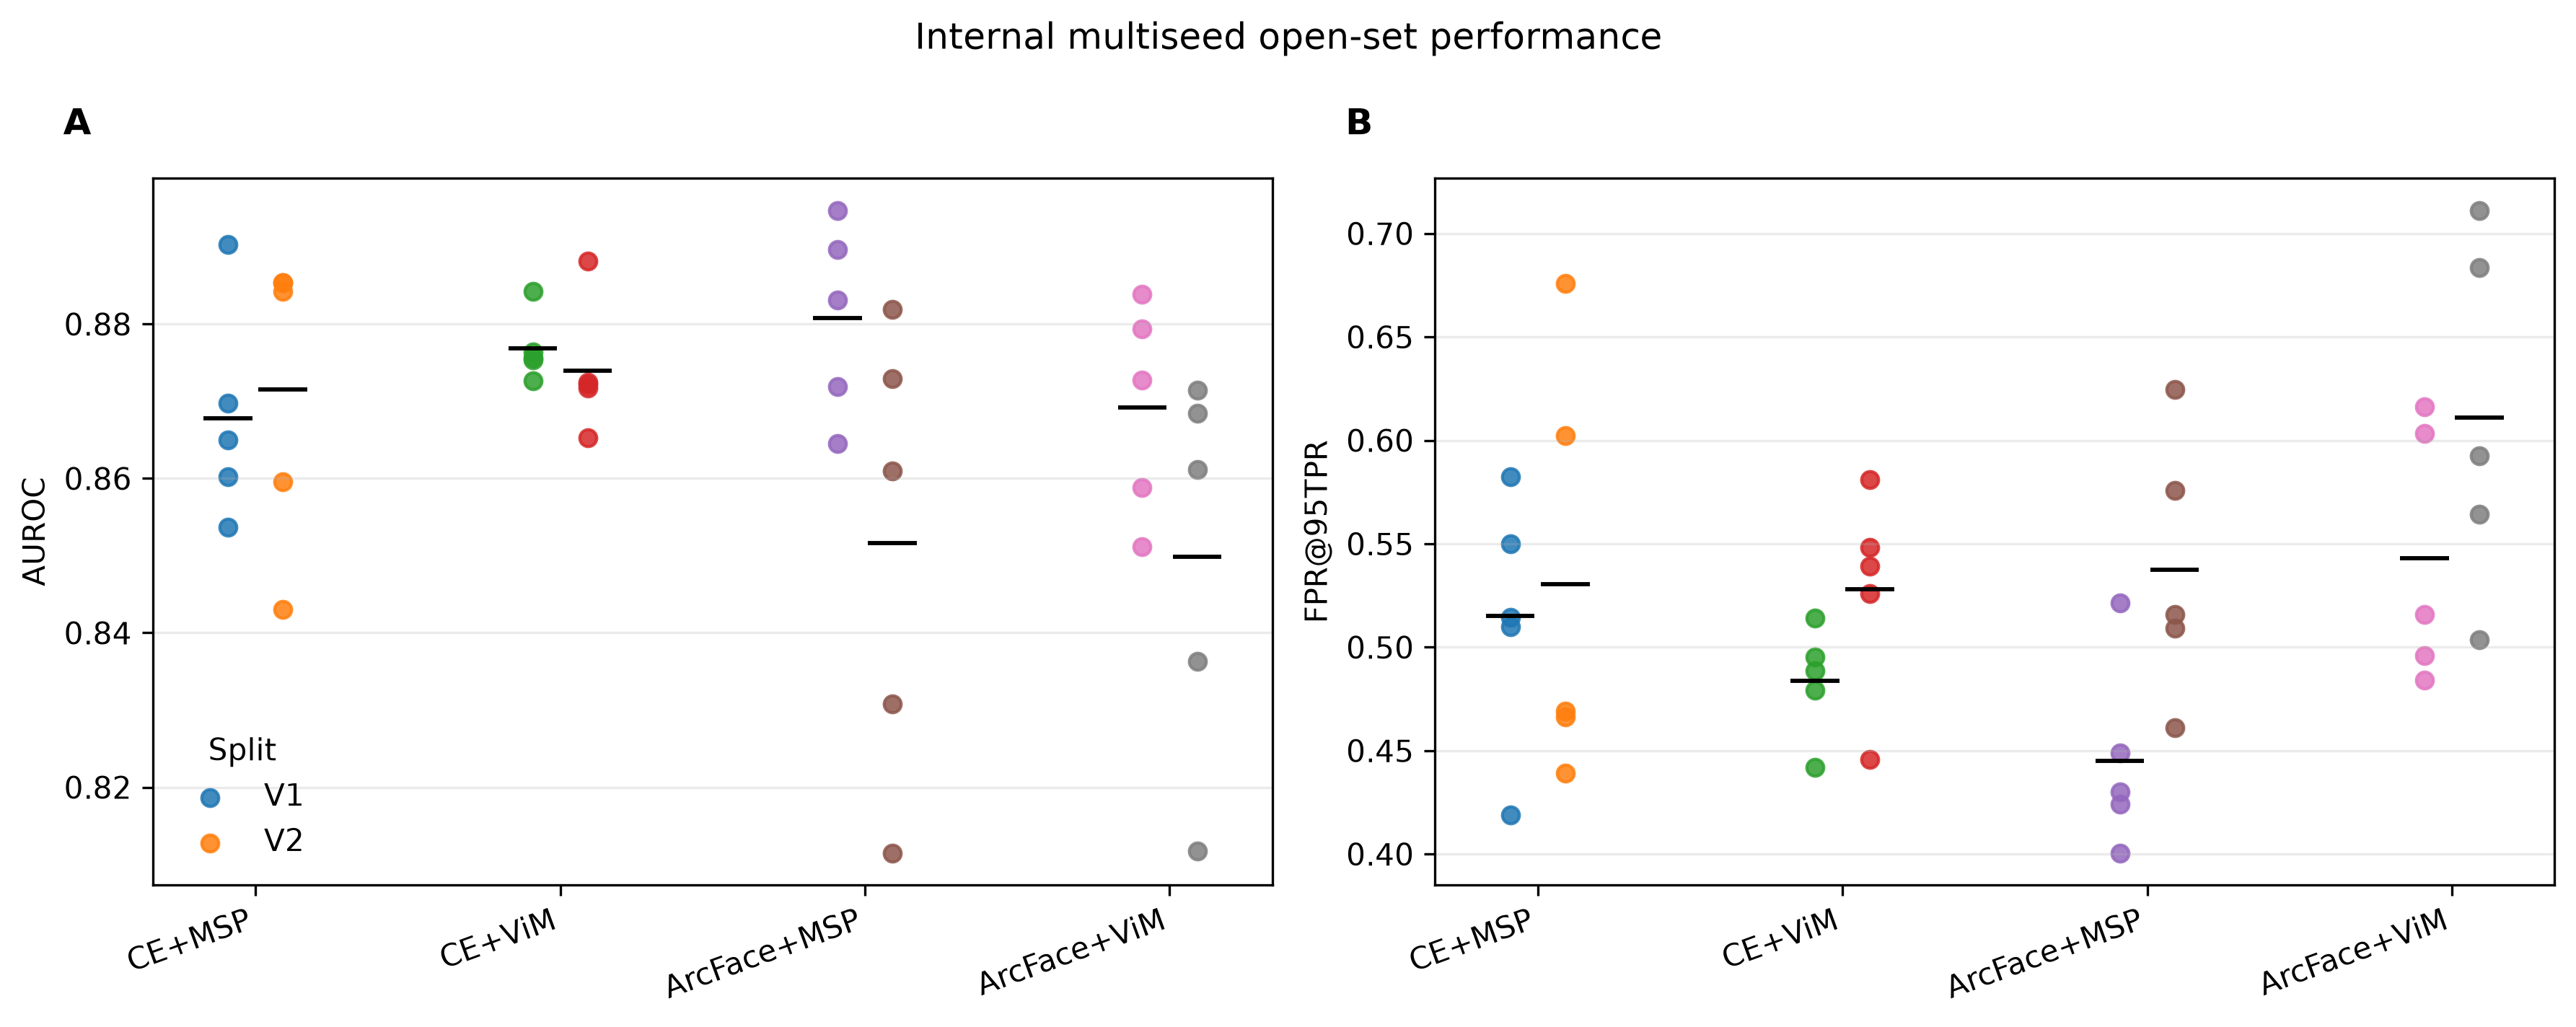
\includegraphics[width=\textwidth]{figure2_internal_performance.png}
\caption{Internal MLL23 open-set performance across five seeds. Points show individual runs and horizontal summaries show seed-level means. Closed-set macro-F1 remains high, while open-set AUROC and FPR@95TPR show larger reliability gaps.}
\label{fig:internal-performance}
\end{figure}

\subsection{Representation-Learning Stability Across Seeds and Splits}

ArcFace improved some known-class geometry summaries but did not reproduce as a robust superior open-set representation. On V1 with MSP, ArcFace reached AUROC 0.881 $\pm$ 0.012, compared with 0.868 $\pm$ 0.014 for CE+MSP. The matched mean ArcFace-minus-CE AUROC delta was +0.013, with four of five seed pairs favorable. However, the frozen interval for this paired delta included zero. The V2 result reversed direction: ArcFace+MSP reached AUROC 0.852 $\pm$ 0.030, whereas CE+MSP reached 0.872 $\pm$ 0.019. The matched V2 delta was -0.020, with only one of five seeds favorable.

The geometric effect of ArcFace was real. Fisher ratio was higher for ArcFace than CE on both V1 and V2: 3.210 $\pm$ 0.181 versus 2.703 $\pm$ 0.065 on V1, and 3.234 $\pm$ 0.323 versus 2.691 $\pm$ 0.092 on V2. Within-class dispersion was much smaller under the normalized angular representation. Yet geometry summaries were weakly associated with MSP AUROC across the 20 internal runs: Fisher ratio had Pearson $r=-0.138$ and Spearman $\rho=0.030$. The result separates known-class geometry from unknown rejection: improving one did not guarantee improving the other.

\begin{figure}[htbp]
\centering
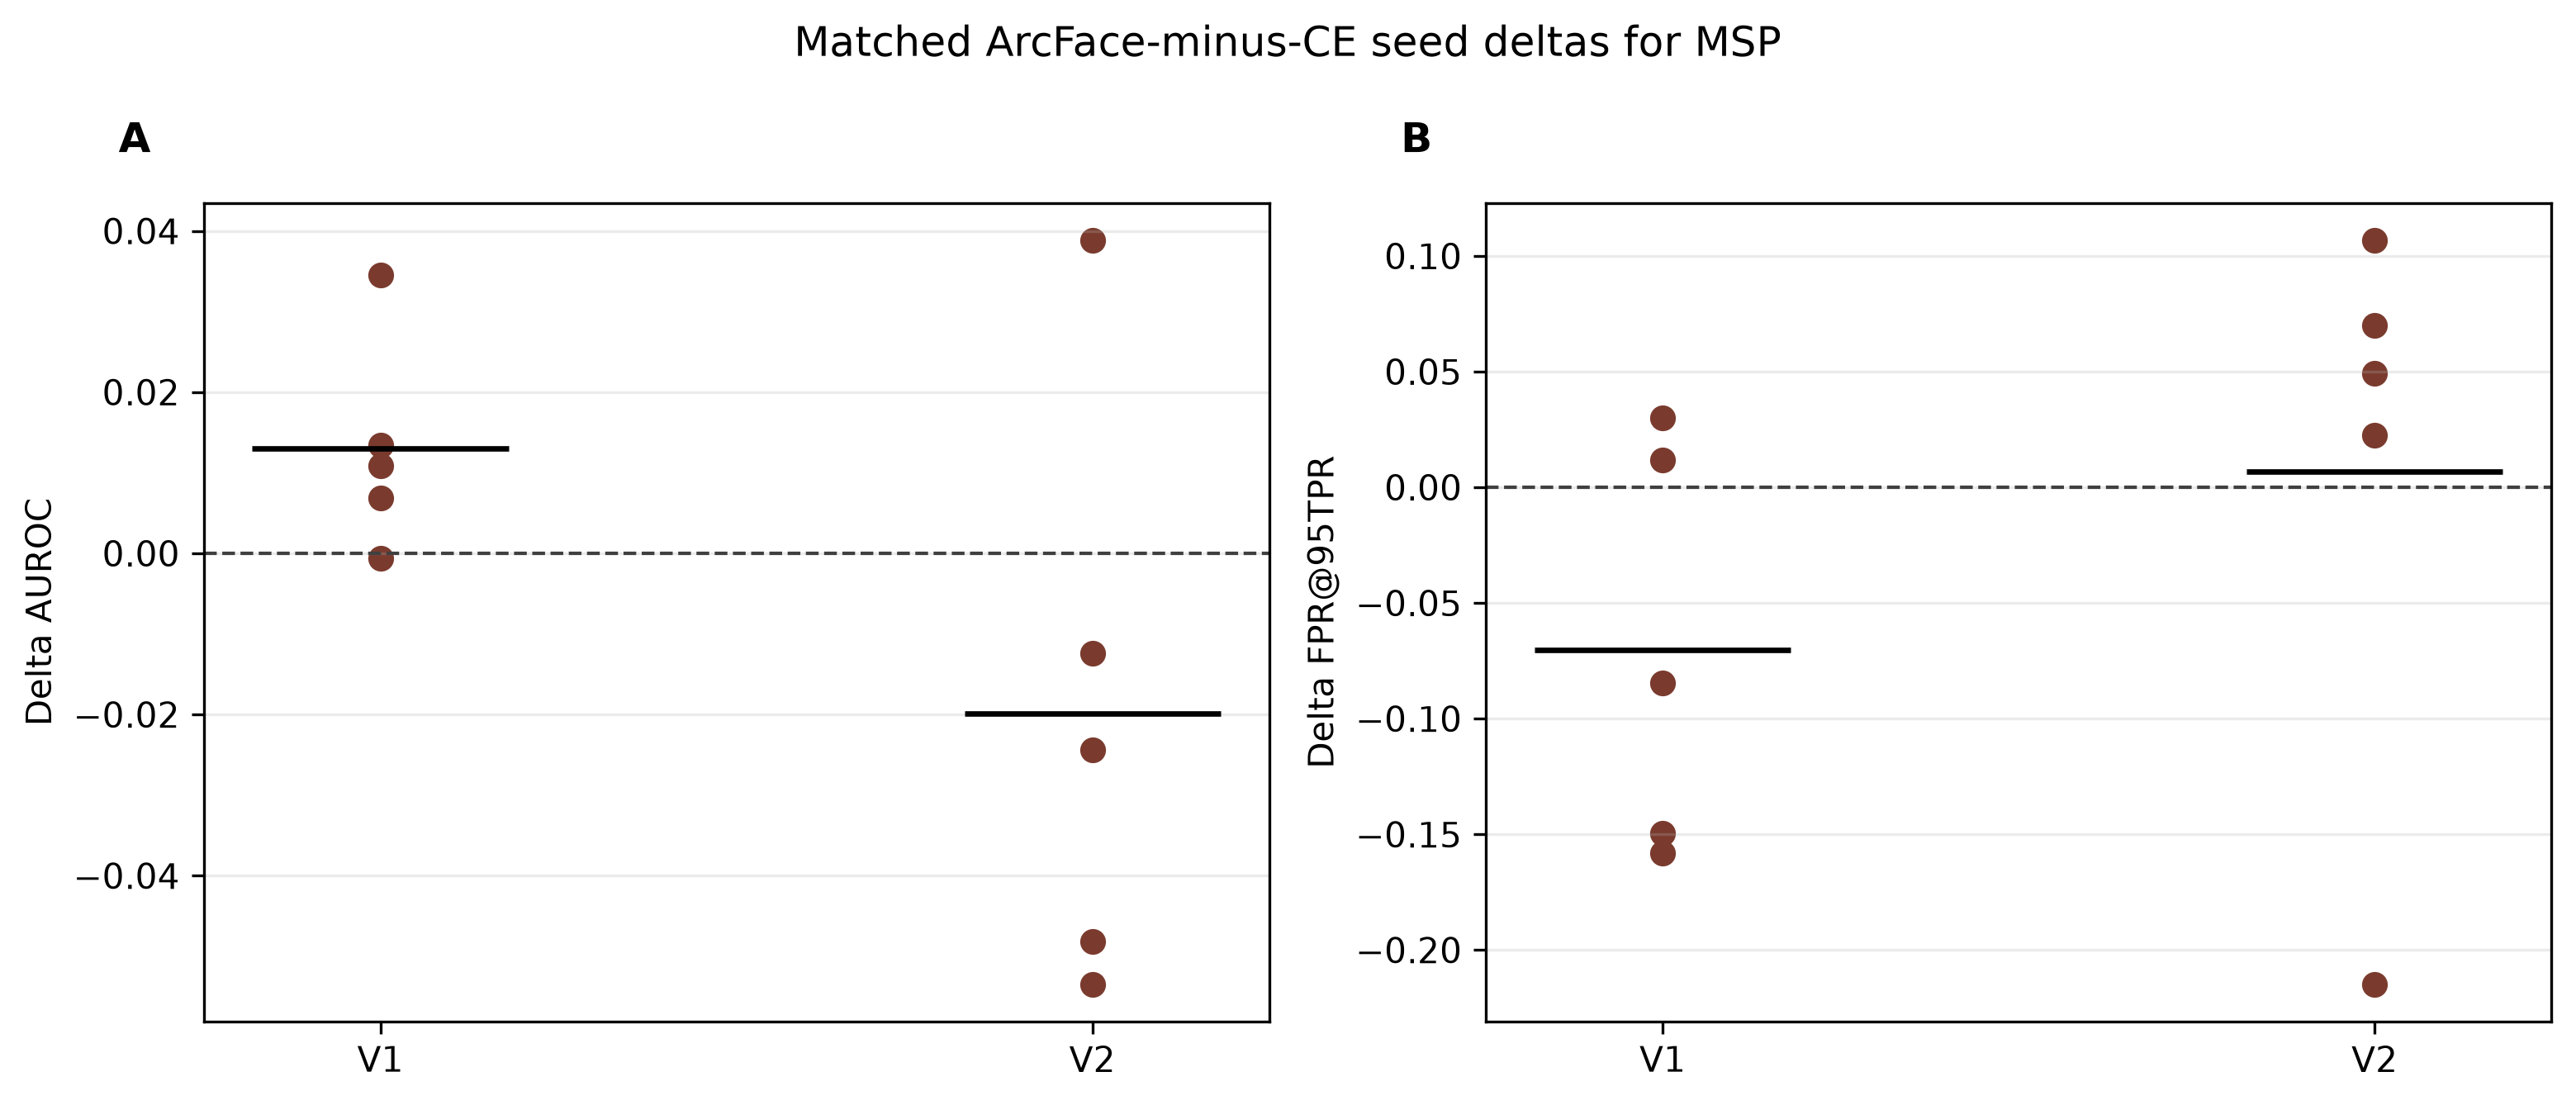
\includegraphics[width=0.92\textwidth]{figure3_arcface_stability.png}
\caption{Matched ArcFace-minus-CE seed deltas for MSP. Positive AUROC deltas favor ArcFace; negative FPR@95TPR deltas favor ArcFace. The V1 trend does not reproduce under V2, so ArcFace is interpreted as an informative ablation rather than a confirmed superior method.}
\label{fig:arcface-stability}
\end{figure}

\subsection{Morphology-Dependent Unknown Rejection}

Unknown rejection difficulty varied strongly by morphology. In the external CE+ViM morphology analysis, the easiest unknowns by mean AUROC were promyelocyte (0.897), myelocyte (0.880), metamyelocyte (0.867), promyelocyte-bilobled (0.856), and erythroblast (0.792). The hardest were neutrophil-band (0.526), monoblast (0.575), myeloblast (0.592), lymphocyte-atypical (0.597), and smudge-cell (0.782). These values should be read as recognition-space measurements, not biological rankings of disease relevance.

The difficult morphologies aligned with dominant known-class attractors. Neutrophil-band samples were assigned most often to segmented neutrophil. Monoblast samples were assigned most often to monocyte. Myeloblast, lymphocyte-atypical, and smudge-cell samples were frequently assigned to lymphocyte. This pattern explains why aggregate AUROC can obscure the most important errors: some unknown morphologies are not generic outliers but close neighbors of the known taxonomy.

\begin{figure}[htbp]
\centering
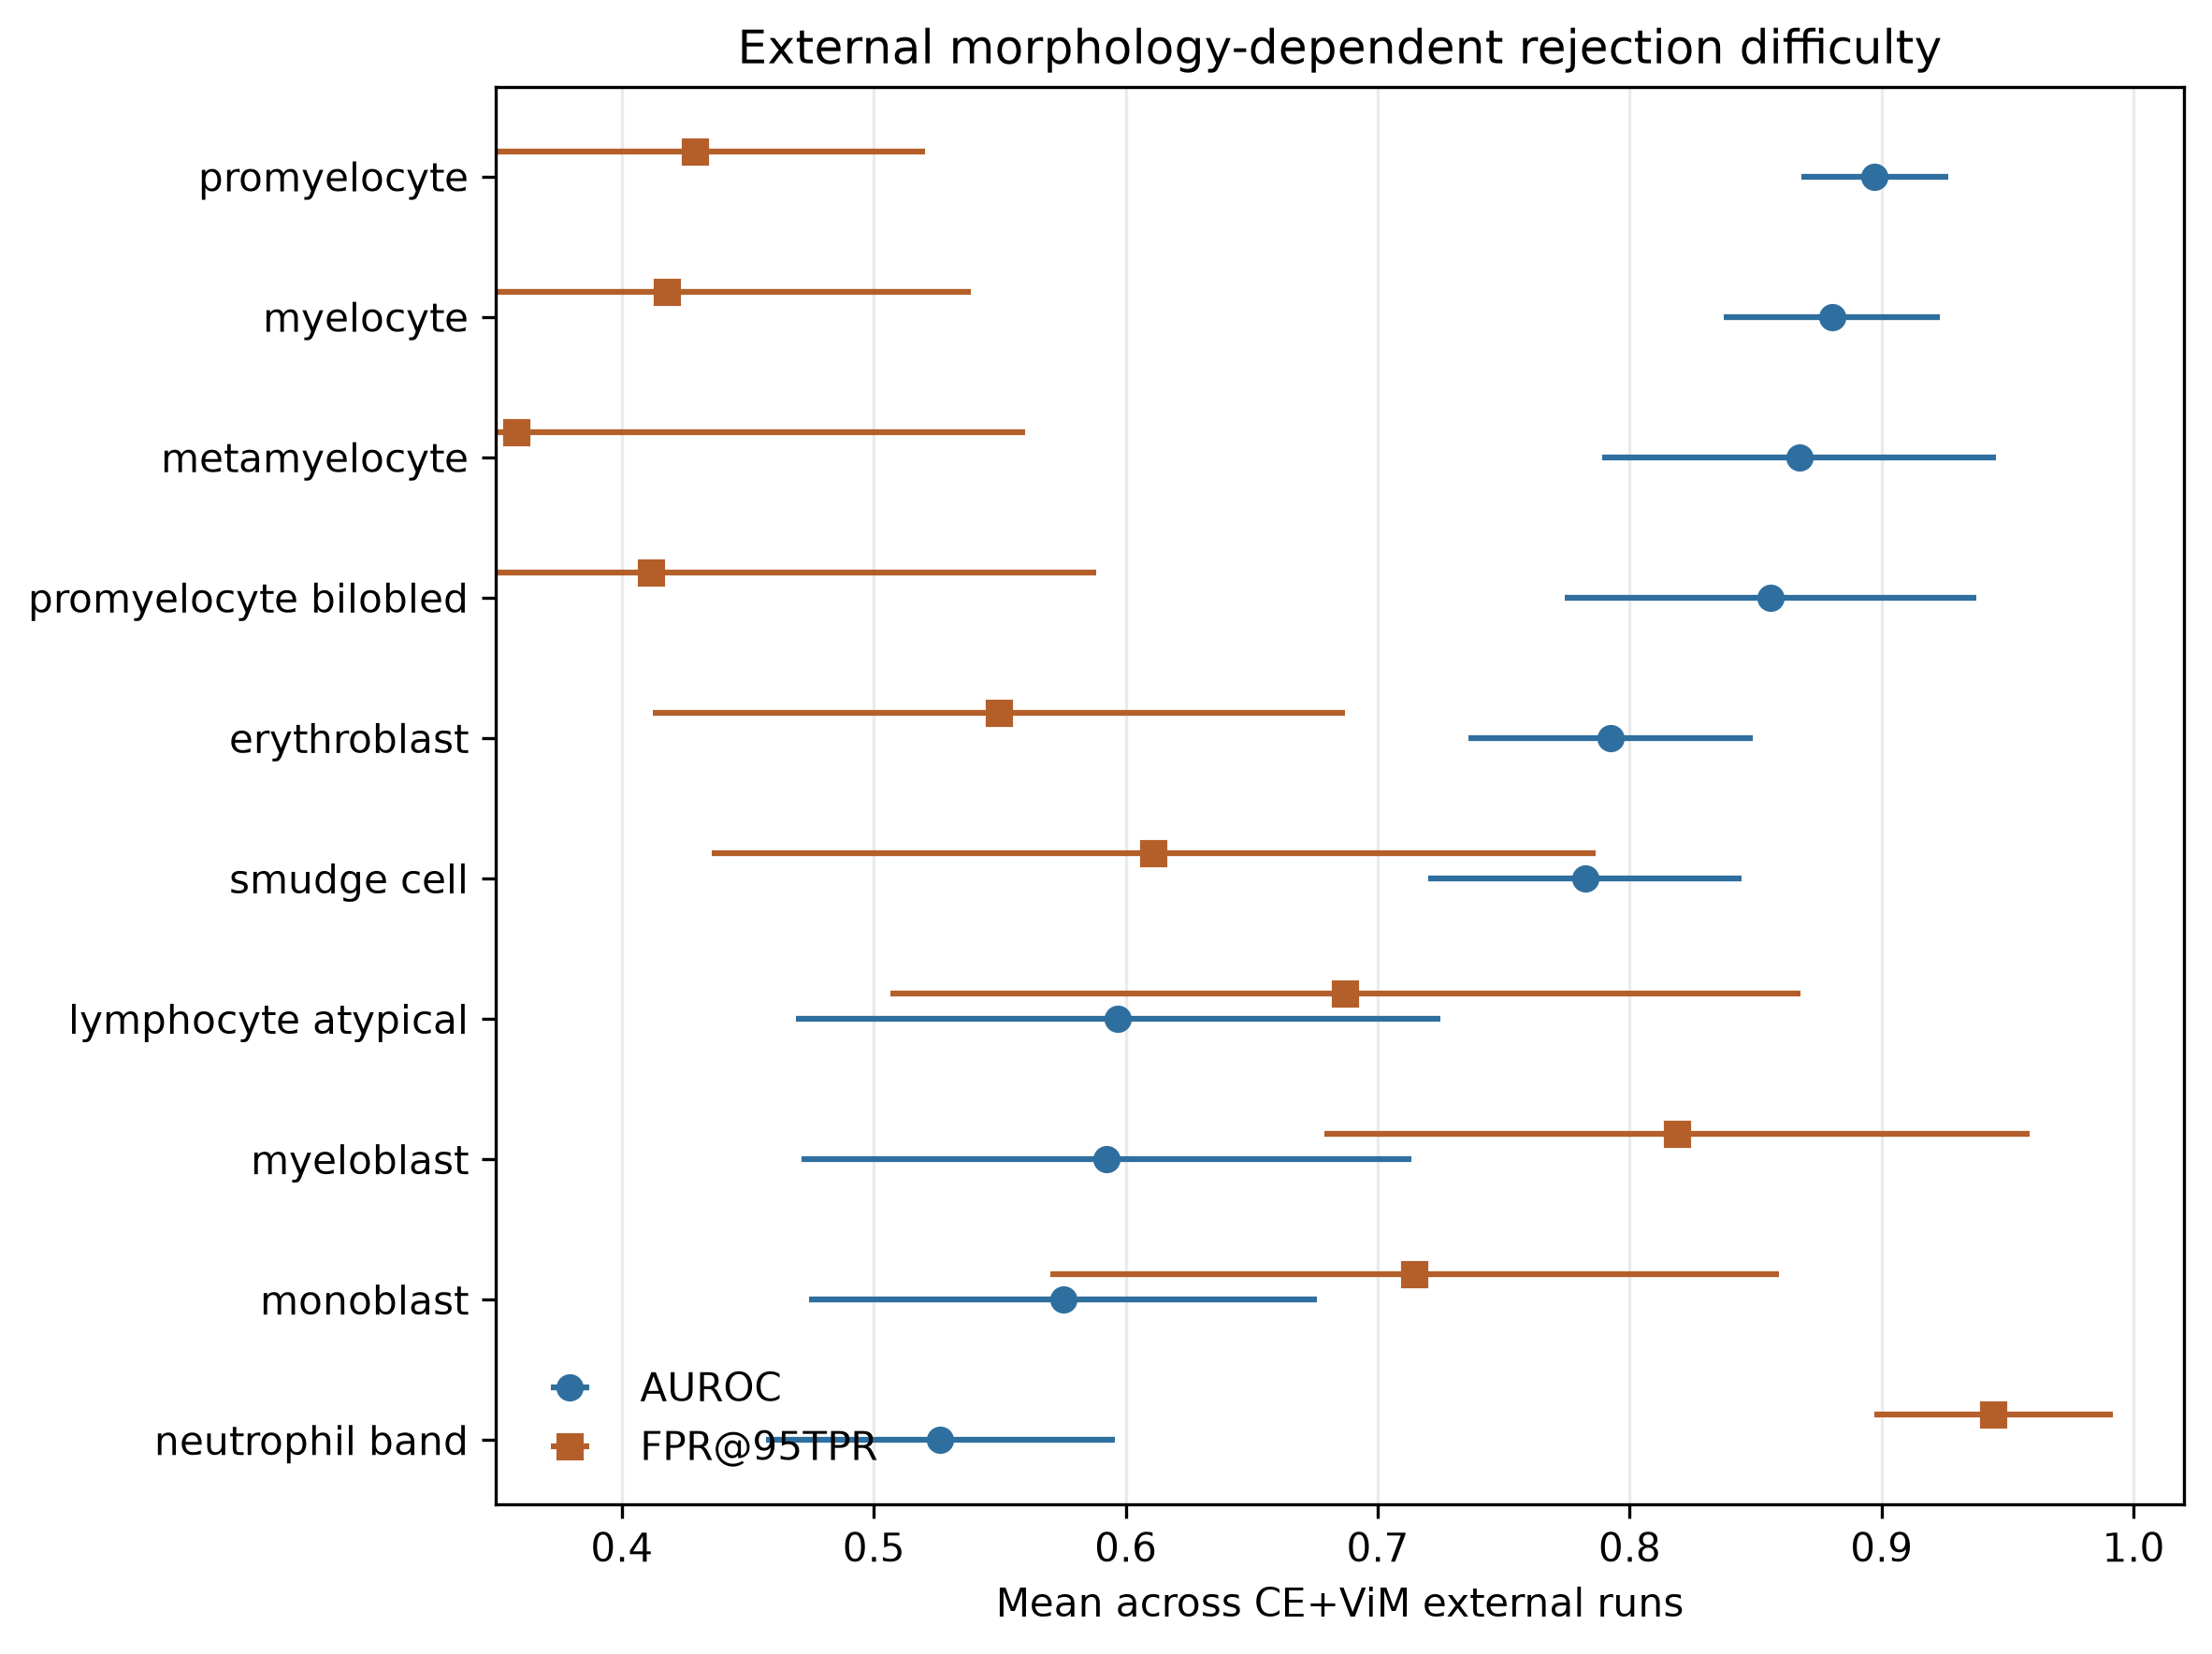
\includegraphics[width=0.86\textwidth]{figure5_external_morphology.png}
\caption{External morphology-dependent unknown detection for CE+ViM. Error bars show standard deviation across frozen CE+ViM external runs. Low AUROC for neutrophil-band, monoblast, myeloblast, and atypical lymphocyte shows that unknown rejection is strongly morphology-dependent.}
\label{fig:external-morphology}
\end{figure}

\begin{figure}[htbp]
\centering
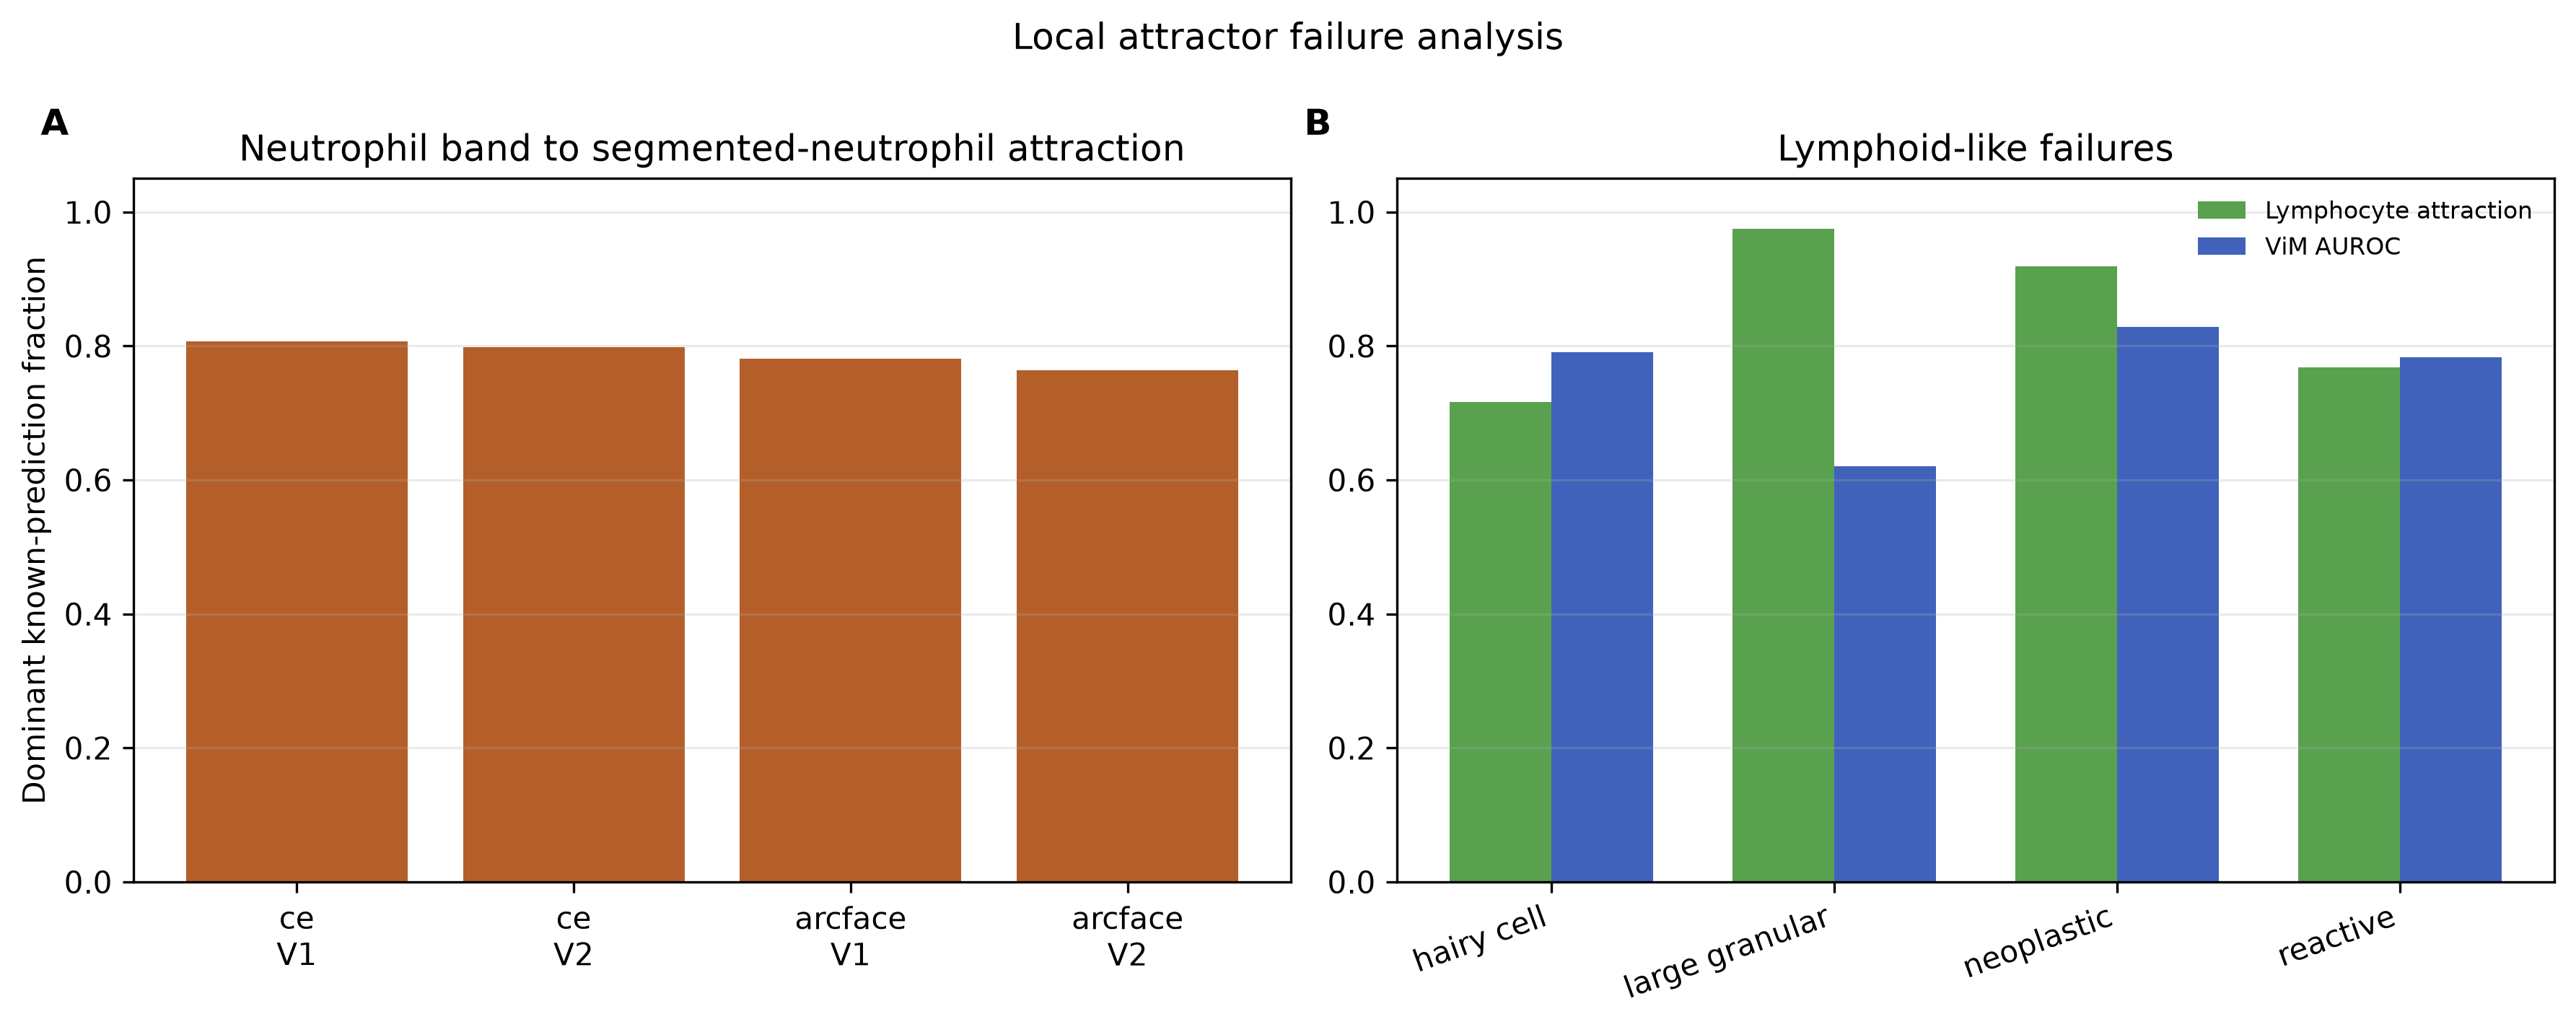
\includegraphics[width=\textwidth]{figure6_failure_cases.png}
\caption{Known-class attractor failure analysis for representative hard unknown morphologies. Neutrophil-band is attracted toward segmented neutrophil, monoblast toward monocyte, and several lymphoid-like unknowns toward lymphocyte.}
\label{fig:failure-cases}
\end{figure}

\subsection{External Validation under Domain Shift}

External closed-set performance degraded substantially on AML-LMU. V1 ArcFace had external closed-set macro-F1 0.755 $\pm$ 0.009, while V1 CE reached 0.711 $\pm$ 0.051. V2 ArcFace reached 0.708 $\pm$ 0.036 and V2 CE reached 0.705 $\pm$ 0.030. These results were far below the internal macro-F1 near 0.97, despite external closed-set accuracy remaining superficially high because the mapped known classes were imbalanced.

External open-set recognition was weaker than internal recognition for every principal system. V1 CE+MSP reached AUROC 0.696 $\pm$ 0.074 and FPR@95TPR 0.796 $\pm$ 0.134. V1 CE+ViM reached AUROC 0.641 $\pm$ 0.090 and FPR@95TPR 0.785 $\pm$ 0.116. V1 ArcFace+MSP reached AUROC 0.690 $\pm$ 0.045 and FPR@95TPR 0.689 $\pm$ 0.107, whereas V1 ArcFace+ViM reached AUROC 0.563 $\pm$ 0.084 and FPR@95TPR 0.879 $\pm$ 0.083.

The V2 external pattern was similarly limited. V2 CE+MSP reached AUROC 0.630 $\pm$ 0.094 and FPR@95TPR 0.887 $\pm$ 0.100. V2 CE+ViM reached AUROC 0.573 $\pm$ 0.123 and FPR@95TPR 0.867 $\pm$ 0.138. V2 ArcFace+MSP reached AUROC 0.696 $\pm$ 0.069 and FPR@95TPR 0.723 $\pm$ 0.162. V2 ArcFace+ViM reached AUROC 0.632 $\pm$ 0.087 and FPR@95TPR 0.851 $\pm$ 0.062.

\begin{table}[htbp]
\centering
\small
\resizebox{\textwidth}{!}{%
\begin{tabular}{l c c c c c}
\toprule
System & Train split & AUROC & FPR@95TPR & OSCR & Closed macro-F1 \\
\midrule
CE+MSP & V1 & 0.696 $\pm$ 0.074 & 0.796 $\pm$ 0.134 & 0.664 $\pm$ 0.068 & 0.711 $\pm$ 0.051 \\
CE+MSP & V2 & 0.630 $\pm$ 0.094 & 0.887 $\pm$ 0.100 & 0.599 $\pm$ 0.081 & 0.705 $\pm$ 0.030 \\
CE+ViM & V1 & 0.641 $\pm$ 0.090 & 0.785 $\pm$ 0.116 & 0.608 $\pm$ 0.078 & 0.711 $\pm$ 0.051 \\
CE+ViM & V2 & 0.573 $\pm$ 0.123 & 0.867 $\pm$ 0.138 & 0.540 $\pm$ 0.107 & 0.705 $\pm$ 0.030 \\
ArcFace+MSP & V1 & 0.690 $\pm$ 0.045 & 0.689 $\pm$ 0.107 & 0.664 $\pm$ 0.043 & 0.755 $\pm$ 0.009 \\
ArcFace+MSP & V2 & 0.696 $\pm$ 0.069 & 0.723 $\pm$ 0.162 & 0.660 $\pm$ 0.075 & 0.708 $\pm$ 0.036 \\
ArcFace+ViM & V1 & 0.563 $\pm$ 0.084 & 0.879 $\pm$ 0.083 & 0.542 $\pm$ 0.080 & 0.755 $\pm$ 0.009 \\
ArcFace+ViM & V2 & 0.632 $\pm$ 0.087 & 0.851 $\pm$ 0.062 & 0.599 $\pm$ 0.086 & 0.708 $\pm$ 0.036 \\
\bottomrule
\end{tabular}
}
\caption{AML-LMU external test-only results. Values are mean $\pm$ standard deviation over five training seeds. No AML-LMU data are used for training, adaptation, calibration, or method selection.}
\label{tab:external}
\end{table}


\begin{figure}[htbp]
\centering
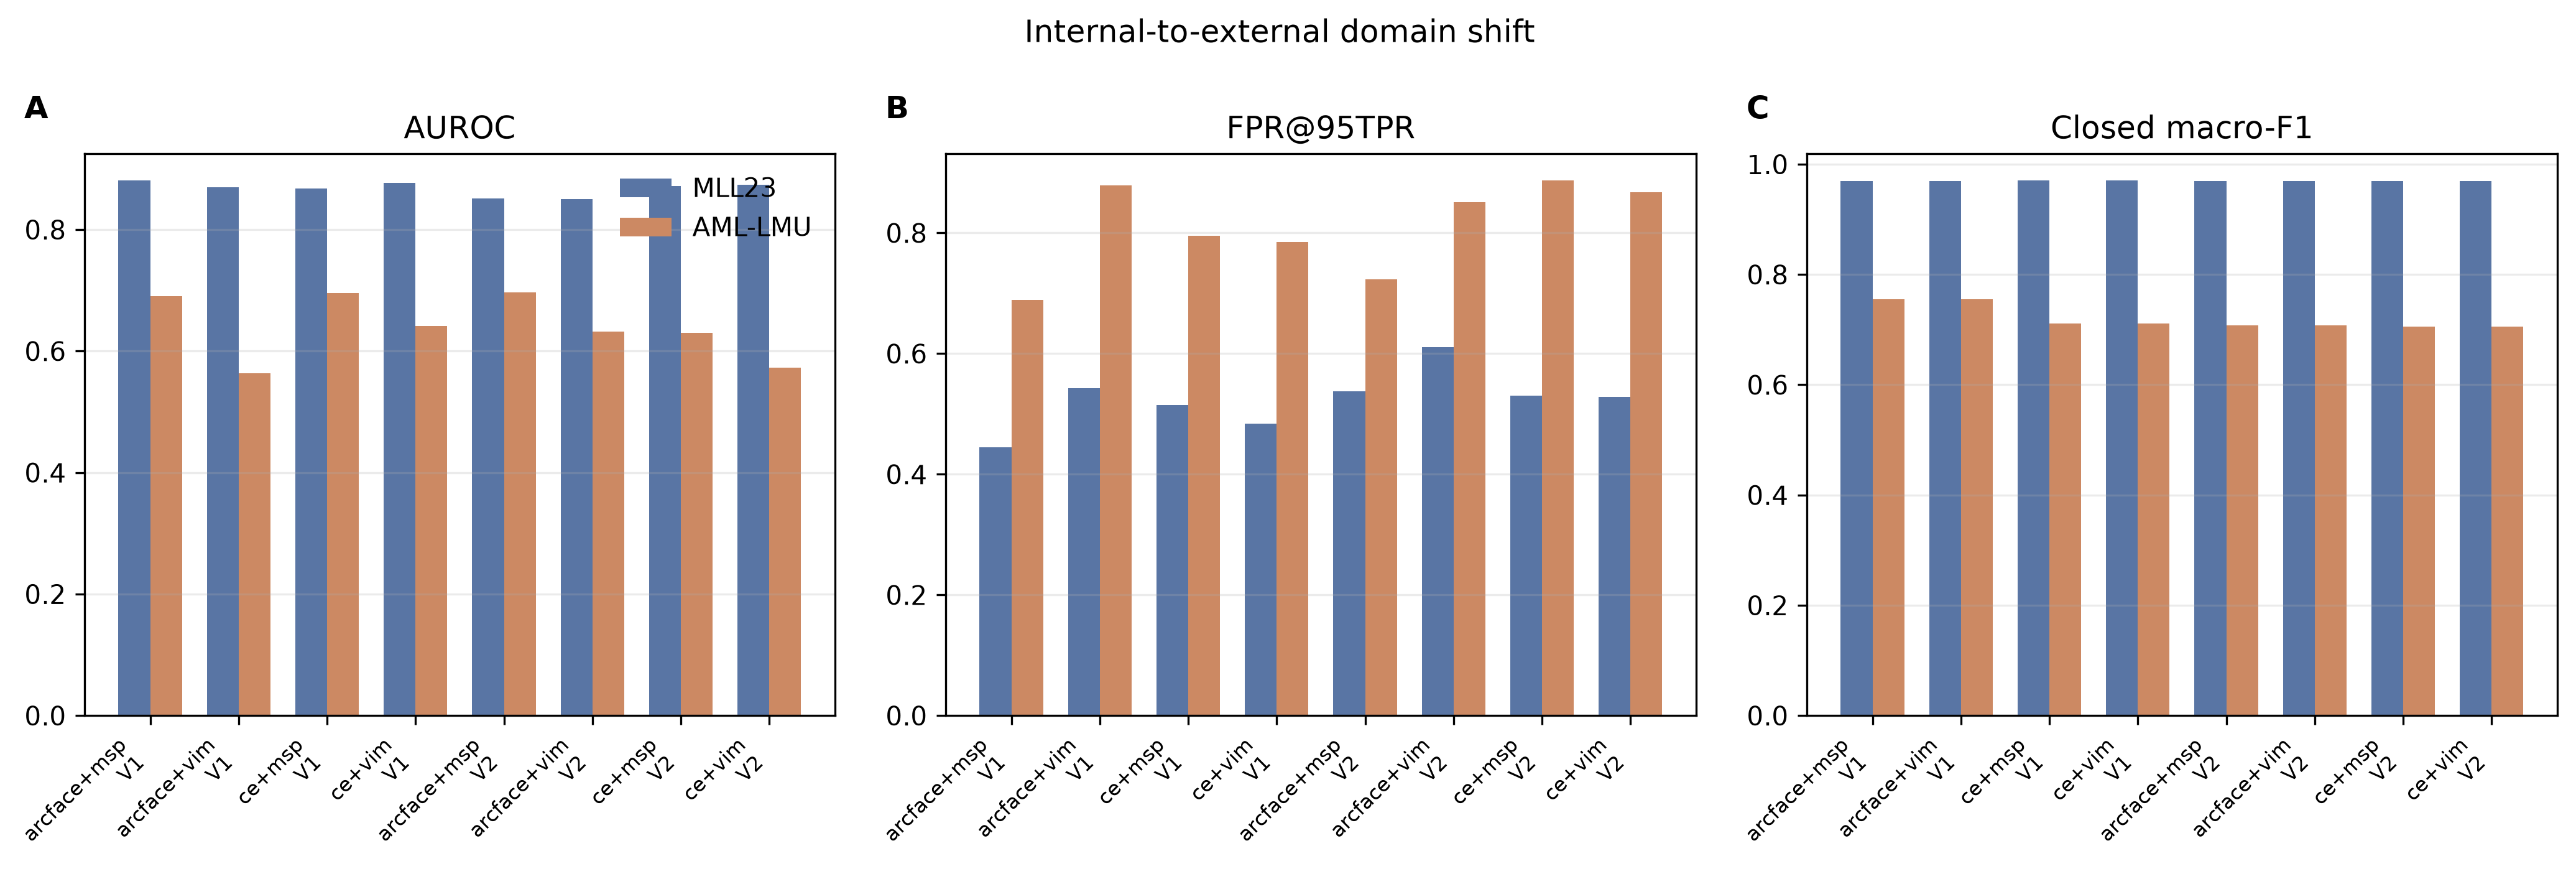
\includegraphics[width=\textwidth]{figure4_domain_shift.png}
\caption{Internal-to-external domain shift for the principal systems. AML-LMU is a test-only domain: no external training, threshold calibration, method selection, PCA fitting, ViM fitting, or preprocessing selection is performed.}
\label{fig:domain-shift}
\end{figure}

\subsection{Internal-to-External Ranking Instability}

Internal method rankings did not transfer cleanly. CE+ViM was the conservative internal-stability baseline, but MSP outperformed ViM by mean external AUROC for both CE and ArcFace across V1 and V2. For example, V1 CE+MSP reached external AUROC 0.696 compared with 0.641 for V1 CE+ViM. V2 CE+MSP reached 0.630 compared with 0.573 for V2 CE+ViM. ArcFace showed a similar MSP advantage externally. The practical external baseline is therefore CE+MSP, while CE+ViM remains the internally stable comparator. The manuscript does not promote a single universal winner.

The magnitude of domain shift was large. For CE+ViM, AUROC dropped from 0.877 to 0.641 on V1 and from 0.874 to 0.573 on V2. FPR@95TPR increased from 0.484 to 0.785 on V1 and from 0.528 to 0.867 on V2. Closed macro-F1 dropped by 0.260 on V1 and 0.264 on V2. These paired changes support the central external-validity conclusion: acquisition and taxonomy-domain differences materially changed both closed-set and open-set behavior.

\subsection{Secondary Topology and Geometry Analysis}

Cubical persistent homology did not provide robust predictive open-set benefit under the evaluated protocol. TDA-only features encoded some class information, with the frozen TDA-only closed macro-F1 reaching approximately 0.828, but open-set AUROC remained approximately 0.55--0.58 for TDA-only variants. Deep+TDA fusion degraded the principal deep baseline rather than improving it. This result is a negative ablation, not a statement that cell morphology has no topological structure.

Vietoris-Rips topology was more useful as a descriptive analysis of learned embeddings. The frozen analysis comprised 500 point-cloud analyses and 1,000 $H_0$/$H_1$ summary rows across internal and external domains, two splits, two representations, five seeds, known classes, and selected hard unknown morphologies. The topology-OSR relationships were weak and inconsistent. For MSP AUROC, mean known $H_1$ max persistence had Pearson $r=0.148$ and Spearman $\rho=0.014$, while Fisher ratio had Pearson $r=-0.138$ and Spearman $\rho=0.030$. These results do not support a predictive or causal topological claim.

\begin{figure}[htbp]
\centering
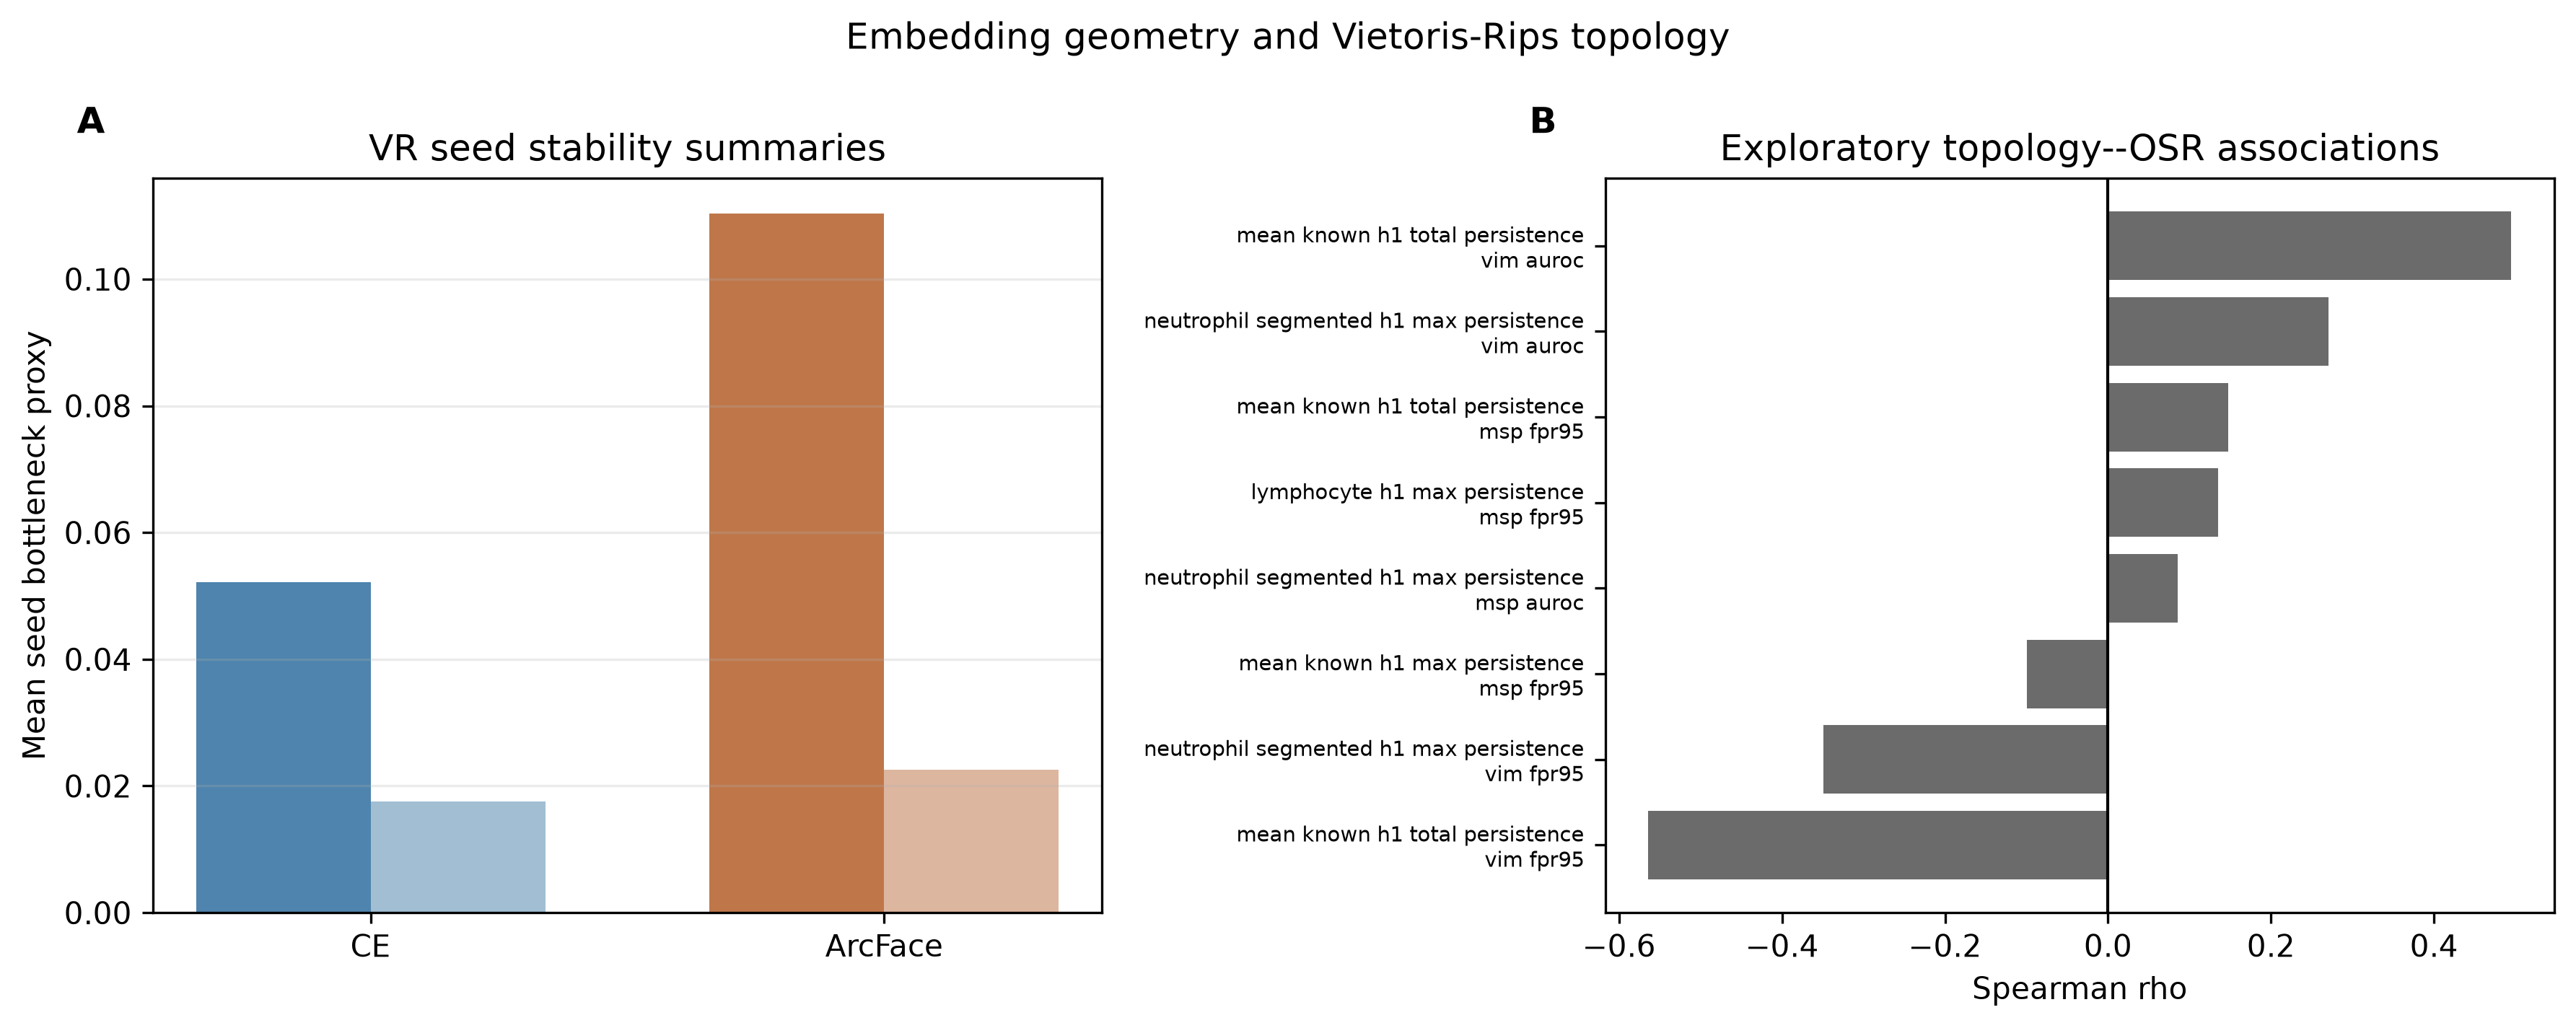
\includegraphics[width=\textwidth]{figure7_topology.png}
\caption{Secondary Vietoris-Rips topology summaries and exploratory associations with OSR metrics. The analysis describes embedding geometry after predictive results are frozen and is not used for model selection, thresholding, or prediction.}
\label{fig:topology}
\end{figure}

\section{Discussion}

\subsection{Closed-Set Performance Is Insufficient Evidence of Open-Set Reliability}

The primary result is the coexistence of strong closed-set leukocyte classification and incomplete open-set reliability. Internally, both CE and ArcFace ResNet18 models achieved macro-F1 near 0.97 on known mature leukocytes. If the evaluation ended there, the systems would appear highly reliable. Open-set metrics changed the interpretation. CE+ViM reached internal AUROC around 0.87, but FPR@95TPR remained near 0.48--0.53. External AUROC then fell to approximately 0.57--0.70 across principal systems, with high FPR@95TPR. These findings show that the ability to classify known leukocytes does not imply the ability to reject unseen morphologies.

This is not a contradiction. Closed-set metrics condition on the assumption that the correct label is in the model's label set. Open-set recognition tests a different behavior: whether an input should be withheld from the known taxonomy. A model can make accurate known-class decisions and still assign a morphologically related unknown sample to the closest known class with high confidence. For hematological morphology, that behavior is expected to be common because unseen classes are often biologically and visually related to known classes rather than arbitrary image corruptions.

\subsection{Morphological Similarity Produces Structured Failure}

The failure analysis indicates that unknown errors are structured by morphology. Neutrophil-band was difficult externally and was dominantly attracted toward segmented neutrophil. Monoblast was dominantly attracted toward monocyte. Myeloblast, atypical lymphocyte, and smudge-cell showed attraction toward lymphocyte in the external CE+ViM analysis. These are not random mistakes. They reflect recognition-space neighborhoods that are plausible under visual morphology, even though the protocol requires these samples to remain outside the known taxonomy.

This observation has two implications. First, aggregate AUROC is necessary but insufficient. A system with acceptable mean performance may still fail on the most clinically or morphologically interesting unknown categories. Second, open-set hematology evaluations should report per-morphology behavior, including known-class attractors and small-class uncertainty. The present study does not claim that these attractors prove biological causality. It claims that open-set errors are morphology-dependent and therefore require morphology-level analysis.

\subsection{Better Known-Class Geometry Does Not Guarantee Better Unknown Separation}

ArcFace is informative precisely because it improved some known-class geometry summaries without producing a robust open-set advantage. The higher Fisher ratio and smaller within-class dispersion show that the representation changed in the intended direction for known classes. However, the V1 MSP AUROC advantage was not confirmed by V2, and the matched-seed evidence did not support a global superiority claim. Externally, ArcFace+MSP was competitive in some comparisons, especially V2, but this does not erase the internal confirmation failure.

The result cautions against a common shortcut: assuming that compact known-class clusters automatically improve unknown rejection. Unknown samples are judged relative to the learned known-class geometry. If an unseen morphology lies near a known class, a more compact or angular representation may still treat it as a confident member of that known neighborhood. The evidence therefore supports a conservative interpretation: ArcFace is a useful representation ablation and a source of insight, not a confirmed method for robust open-set leukocyte recognition.

\subsection{External Domain Shift Changes the Problem}

AML-LMU is the decisive stress test in the paper. It differs from MLL23 in source, acquisition context, image dimensions, class composition, and source taxonomy. The test-only protocol prevents external adaptation from obscuring the generalization question. Under this design, all principal systems degraded. Closed macro-F1 fell by roughly 0.21--0.26 depending on representation and split, and open-set AUROC fell for every system. The method ranking also changed: ViM was stable internally but MSP was stronger externally in the principal CE and ArcFace comparisons.

This ranking instability matters for research practice. If a method is selected solely because it performs best internally, the selection may not transfer to a new acquisition domain. Conversely, if a method looks strong externally after many external tuning choices, it may no longer be a clean test of generalization. The present study chooses the stricter route: external data remain untouched until final evaluation. The resulting performance is not flattering, but it is scientifically useful because it measures a realistic failure mode.

\subsection{What Persistent Homology Reveals and Does Not Reveal}

Persistent homology has a disciplined but secondary role. Cubical persistent homology was tested as a predictive feature family and did not provide robust complementary unknown-detection utility. The negative result should remain in the paper because it prevents the title and framing from implying an unsupported topology-based method. It also documents that image-derived topology, as implemented in the frozen experiments, did not solve the open-set problem.

Vietoris-Rips persistent homology is different. It describes the topology of learned embedding clouds after the predictive experiments are fixed. The observed seed, split, and domain variation may help characterize representation behavior, but the topology-OSR correlations are weak and inconsistent. The study therefore avoids causal claims. Topology may be useful for future exploratory diagnostics, but the present evidence does not support using it as a predictor of open-set reliability.

\subsection{Implications for Evaluation}

The results support a conservative evaluation checklist for hematological morphology systems. Unknown classes should be defined before metrics are produced. Unknown samples should remain test-only. Exact and near-duplicate leakage should be audited, and patient-level validation should not be claimed when patient identifiers are unavailable. Results should be reported across seeds, externally where possible, and per unknown morphology. Claims should distinguish known-class classification, open-set recognition, and patient-level diagnosis.

This manuscript is therefore best positioned as a rigorous empirical study rather than a new architecture paper. Its contribution is not that CE, ArcFace, ViM, MSP, or persistent homology is the final answer. Its contribution is the evidence that a plausible closed-set leukocyte classifier can fail in structured ways when the taxonomy is incomplete and the acquisition domain changes.

The study also argues for a different style of reporting in biomedical morphology benchmarks. A single same-source accuracy number is easy to communicate, but it can hide whether the model has learned a robust morphology representation or a narrower source-specific decision rule. Reporting seed variation, split sensitivity, external transfer, and morphology-level unknown behavior makes the story less tidy, but it better reflects the reliability question that arises when models are reused outside their original label inventory. This is particularly important for open-set settings, where the most consequential behavior may be the decision not to assign a known class.

Finally, the results clarify the role of negative evidence. The ArcFace and persistent-homology analyses did not produce a simple improvement story, but they prevent misleading conclusions. ArcFace shows that better known-class geometry is not equivalent to better unknown rejection. Cubical persistent homology shows that the evaluated image-topology descriptors did not rescue open-set performance. Vietoris-Rips summaries show that embedding topology can be described without being promoted as a predictor. Keeping these findings in the manuscript makes the evaluation more reproducible and less vulnerable to selective reporting.

\section{Limitations}

Several limitations constrain the interpretation of this study. First, MLL23 is the single internal dataset and AML-LMU is the single external domain. Additional independent datasets would be needed to estimate the range of domain-shift behavior across scanners, stains, laboratories, annotation policies, and patient populations. Second, reliable patient or acquisition-group identifiers are unavailable in the working MLL23 manifests. The V2 split is a conservative exact and near-duplicate sensitivity analysis, not patient-level validation. AML-LMU documents subject counts in the source collection, but patient identifiers were not available in the audited fields used for this project.

Third, the unknown classes are defined by the protocol. They are outside the known training taxonomy, but they do not define malignancy, leukemia, abnormal diagnosis, or a positive clinical finding. Fourth, the class distribution is imbalanced in both internal and external data. This motivates macro-F1, balanced accuracy, per-morphology results, and open-set metrics, but imbalance still affects uncertainty around small external unknown classes such as atypical lymphocytes, metamyelocytes, monoblasts, and smudge cells.

Fifth, the model family is limited to ImageNet-pretrained ResNet18 variants with frozen training settings. The study uses five seeds, which is stronger than a single-run report but not exhaustive. Sixth, ArcFace is evaluated with one frozen margin and scale. Further tuning could change results, but tuning after seeing confirmatory outcomes would reopen method selection and weaken the frozen evaluation design. Seventh, the internal unknown set was inspected during prior analysis, so internal explanatory findings should not be treated as independent discovery. The external test-only analysis is therefore especially important.

Eighth, no external adaptation is performed. This strengthens the external validation claim but does not estimate the best possible performance after domain adaptation, stain normalization, external calibration, or target-domain fine-tuning. Ninth, persistent-homology conclusions are limited to the evaluated filtrations, vectorizers, fusion designs, sample sizes, and summary statistics. They should not be generalized to all topological methods. Finally, the study is a research evaluation on public datasets, not a prospective clinical workflow evaluation, not a patient-level diagnostic task, and not a guarantee that dataset-defined unknowns cover the full diversity of real-world hematological morphology.

\section{Conclusion}

This study evaluates open-set recognition of unseen leukocyte morphologies under a frozen taxonomy and external domain shift. The main conclusion is that high closed-set performance is not enough: ResNet18 models reached internal known-class macro-F1 near 0.97, but unknown rejection remained imperfect, morphology-dependent, and substantially weaker under AML-LMU external validation. Difficult unknowns were not uniformly distributed; they were attracted toward plausible known classes such as segmented neutrophil, monocyte, and lymphocyte.

ArcFace improved some known-class geometry summaries but did not reproduce as a robust superior open-set representation across seeds and split protocols. Cubical persistent homology provided negative predictive evidence, and Vietoris-Rips topology remained explanatory rather than causal or predictive. The most defensible message is therefore evaluation-centered: leukocyte morphology classifiers should be tested with explicit taxonomy freezes, test-only unknown morphologies, seed and split sensitivity, morphology-level failure analysis, and independent external validation before closed-set performance is interpreted as evidence of open-set reliability.

\section*{Declarations}

\subsection*{Data Availability}

This manuscript uses public datasets. MLL23 is available through Zenodo at DOI \href{https://doi.org/10.5281/zenodo.14277609}{10.5281/zenodo.14277609} and is described in Scientific Data \cite{mll23_nature_2025,mll23_zenodo_2024}. AML-Cytomorphology\_LMU is available through The Cancer Imaging Archive at DOI \href{https://doi.org/10.7937/tcia.2019.36f5o9ld}{10.7937/tcia.2019.36f5o9ld} \cite{aml_lmu_tcia_2019}. Raw datasets are not redistributed with this manuscript. Manuscript-level summaries are derived from frozen local artifacts listed in the traceability file.

\subsection*{Code Availability}

The analysis code is maintained in the project repository used to prepare this manuscript. A public archival repository URL and software release identifier were not verified during this editorial revision and should be supplied by the author before journal submission.

\subsection*{Author Contributions}

G. Álvarez Sánchez is listed as the manuscript author in the current LaTeX source. A final CRediT author-contribution statement should be confirmed by the author before submission.

\subsection*{Funding}

Funding information was not available in the reviewed repository materials and requires author confirmation before submission.

\subsection*{Declaration of Competing Interest}

A competing-interest declaration was not available in the reviewed repository materials and requires author confirmation before submission.

\subsection*{Ethics Statement}

This study is a secondary analysis of public, de-identified image datasets. The MLL23 source article reports ethics approval and consent information for its dataset \cite{mll23_nature_2025}. AML-Cytomorphology\_LMU is distributed by The Cancer Imaging Archive. No new human participant data were collected for this manuscript. Any institution-specific ethics wording should be confirmed by the author before submission.

\subsection*{Acknowledgments}

No acknowledgments were available in the reviewed repository materials.


\bibliographystyle{unsrt}
\bibliography{references}

\end{document}
